\documentclass{book}
\usepackage[a4paper,top=2.5cm,bottom=2.5cm,left=2.5cm,right=2.5cm]{geometry}
\usepackage{makeidx}
\usepackage{natbib}
\usepackage{graphicx}
\usepackage{multicol}
\usepackage{float}
\usepackage{listings}
\usepackage{color}
\usepackage{ifthen}
\usepackage[table]{xcolor}
\usepackage{textcomp}
\usepackage{alltt}
\usepackage{ifpdf}
\ifpdf
\usepackage[pdftex,
            pagebackref=true,
            colorlinks=true,
            linkcolor=blue,
            unicode
           ]{hyperref}
\else
\usepackage[ps2pdf,
            pagebackref=true,
            colorlinks=true,
            linkcolor=blue,
            unicode
           ]{hyperref}
\usepackage{pspicture}
\fi
\usepackage[utf8]{inputenc}
\usepackage{mathptmx}
\usepackage[scaled=.90]{helvet}
\usepackage{courier}
\usepackage{sectsty}
\usepackage{amssymb}
\usepackage[titles]{tocloft}
\usepackage{doxygen}
\lstset{language=C++,inputencoding=utf8,basicstyle=\footnotesize,breaklines=true,breakatwhitespace=true,tabsize=8,numbers=left }
\makeindex
\setcounter{tocdepth}{3}
\renewcommand{\footrulewidth}{0.4pt}
\renewcommand{\familydefault}{\sfdefault}
\hfuzz=15pt
\setlength{\emergencystretch}{15pt}
\hbadness=750
\tolerance=750
\begin{document}
\hypersetup{pageanchor=false,citecolor=blue}
\begin{titlepage}
\vspace*{7cm}
\begin{center}
{\Large Super\-Guy }\\
\vspace*{1cm}
{\large Generated by Doxygen 1.8.1.2}\\
\vspace*{0.5cm}
{\small Mon Mar 25 2013 11:31:47}\\
\end{center}
\end{titlepage}
\clearemptydoublepage
\pagenumbering{roman}
\tableofcontents
\clearemptydoublepage
\pagenumbering{arabic}
\hypersetup{pageanchor=true,citecolor=blue}
\chapter{Super\-Guy}
\label{index}\hypertarget{index}{}\hypertarget{index_intro_sec}{}\section{Introduction}\label{index_intro_sec}
A Super\-Mario themed clone with 8 bit Music.\hypertarget{index_install_sec}{}\section{Installation}\label{index_install_sec}
\hypertarget{index_step1}{}\subsection{Step 1\-: Download}\label{index_step1}

\chapter{Class Index}
\section{Class Hierarchy}
This inheritance list is sorted roughly, but not completely, alphabetically\-:\begin{DoxyCompactList}
\item \contentsline{section}{dvar}{\pageref{classdvar}}{}
\item \contentsline{section}{dvar\-\_\-value}{\pageref{uniondvar__value}}{}
\item \contentsline{section}{dvar\-Manager}{\pageref{classdvar_manager}}{}
\item \contentsline{section}{enemy\-Ant}{\pageref{classenemy_ant}}{}
\item \contentsline{section}{enemy\-Duck}{\pageref{classenemy_duck}}{}
\item \contentsline{section}{engine}{\pageref{classengine}}{}
\item \contentsline{section}{event\-Handler}{\pageref{classevent_handler}}{}
\item \contentsline{section}{log}{\pageref{classlog}}{}
\item \contentsline{section}{state\-Machine}{\pageref{classstate_machine}}{}
\begin{DoxyCompactList}
\item \contentsline{section}{Game\-Over}{\pageref{class_game_over}}{}
\item \contentsline{section}{Intro}{\pageref{class_intro}}{}
\item \contentsline{section}{Over\-World}{\pageref{class_over_world}}{}
\item \contentsline{section}{Stage1}{\pageref{class_stage1}}{}
\item \contentsline{section}{Title}{\pageref{class_title}}{}
\end{DoxyCompactList}
\item \contentsline{section}{texture}{\pageref{classtexture}}{}
\end{DoxyCompactList}

\chapter{Class Index}
\section{Class List}
Here are the classes, structs, unions and interfaces with brief descriptions\-:\begin{DoxyCompactList}
\item\contentsline{section}{\hyperlink{classdvar}{dvar} }{\pageref{classdvar}}{}
\item\contentsline{section}{\hyperlink{uniondvar__value}{dvar\-\_\-value} }{\pageref{uniondvar__value}}{}
\item\contentsline{section}{\hyperlink{classdvar_manager}{dvar\-Manager} }{\pageref{classdvar_manager}}{}
\item\contentsline{section}{\hyperlink{classenemy_ant}{enemy\-Ant} }{\pageref{classenemy_ant}}{}
\item\contentsline{section}{\hyperlink{classenemy_duck}{enemy\-Duck} }{\pageref{classenemy_duck}}{}
\item\contentsline{section}{\hyperlink{classengine}{engine} }{\pageref{classengine}}{}
\item\contentsline{section}{\hyperlink{classevent_handler}{event\-Handler} }{\pageref{classevent_handler}}{}
\item\contentsline{section}{\hyperlink{class_game_over}{Game\-Over} }{\pageref{class_game_over}}{}
\item\contentsline{section}{\hyperlink{class_intro}{Intro} }{\pageref{class_intro}}{}
\item\contentsline{section}{\hyperlink{classlog}{log} }{\pageref{classlog}}{}
\item\contentsline{section}{\hyperlink{class_over_world}{Over\-World} }{\pageref{class_over_world}}{}
\item\contentsline{section}{\hyperlink{class_stage1}{Stage1} }{\pageref{class_stage1}}{}
\item\contentsline{section}{\hyperlink{classstate_machine}{state\-Machine} }{\pageref{classstate_machine}}{}
\item\contentsline{section}{\hyperlink{classtexture}{texture} }{\pageref{classtexture}}{}
\item\contentsline{section}{\hyperlink{class_title}{Title} }{\pageref{class_title}}{}
\end{DoxyCompactList}

\chapter{File Index}
\section{File List}
Here is a list of all files with brief descriptions\-:\begin{DoxyCompactList}
\item\contentsline{section}{/home/ludkiller/projects/\-Super\-Guy/src/\hyperlink{log_8cpp}{log.\-cpp} }{\pageref{log_8cpp}}{}
\item\contentsline{section}{/home/ludkiller/projects/\-Super\-Guy/src/\hyperlink{log_8h}{log.\-h} }{\pageref{log_8h}}{}
\item\contentsline{section}{/home/ludkiller/projects/\-Super\-Guy/src/\hyperlink{main_8cpp}{main.\-cpp} }{\pageref{main_8cpp}}{}
\item\contentsline{section}{/home/ludkiller/projects/\-Super\-Guy/src/enemy/\hyperlink{_a_i_entity_8cpp}{A\-I\-Entity.\-cpp} }{\pageref{_a_i_entity_8cpp}}{}
\item\contentsline{section}{/home/ludkiller/projects/\-Super\-Guy/src/enemy/\hyperlink{_a_i_entity_8h}{A\-I\-Entity.\-h} }{\pageref{_a_i_entity_8h}}{}
\item\contentsline{section}{/home/ludkiller/projects/\-Super\-Guy/src/enemy/\hyperlink{enemy_ant_8cpp}{enemy\-Ant.\-cpp} }{\pageref{enemy_ant_8cpp}}{}
\item\contentsline{section}{/home/ludkiller/projects/\-Super\-Guy/src/enemy/\hyperlink{enemy_ant_8h}{enemy\-Ant.\-h} }{\pageref{enemy_ant_8h}}{}
\item\contentsline{section}{/home/ludkiller/projects/\-Super\-Guy/src/enemy/\hyperlink{enemy_duck_8cpp}{enemy\-Duck.\-cpp} }{\pageref{enemy_duck_8cpp}}{}
\item\contentsline{section}{/home/ludkiller/projects/\-Super\-Guy/src/enemy/\hyperlink{enemy_duck_8h}{enemy\-Duck.\-h} }{\pageref{enemy_duck_8h}}{}
\item\contentsline{section}{/home/ludkiller/projects/\-Super\-Guy/src/engine/\hyperlink{dvar_8cpp}{dvar.\-cpp} }{\pageref{dvar_8cpp}}{}
\item\contentsline{section}{/home/ludkiller/projects/\-Super\-Guy/src/engine/\hyperlink{dvar_8h}{dvar.\-h} }{\pageref{dvar_8h}}{}
\item\contentsline{section}{/home/ludkiller/projects/\-Super\-Guy/src/engine/\hyperlink{dvar_manager_8cpp}{dvar\-Manager.\-cpp} }{\pageref{dvar_manager_8cpp}}{}
\item\contentsline{section}{/home/ludkiller/projects/\-Super\-Guy/src/engine/\hyperlink{dvar_manager_8h}{dvar\-Manager.\-h} }{\pageref{dvar_manager_8h}}{}
\item\contentsline{section}{/home/ludkiller/projects/\-Super\-Guy/src/engine/\hyperlink{engine_8cpp}{engine.\-cpp} }{\pageref{engine_8cpp}}{}
\item\contentsline{section}{/home/ludkiller/projects/\-Super\-Guy/src/engine/\hyperlink{engine_8h}{engine.\-h} }{\pageref{engine_8h}}{}
\item\contentsline{section}{/home/ludkiller/projects/\-Super\-Guy/src/engine/\hyperlink{texture_8cpp}{texture.\-cpp} }{\pageref{texture_8cpp}}{}
\item\contentsline{section}{/home/ludkiller/projects/\-Super\-Guy/src/engine/\hyperlink{texture_8h}{texture.\-h} }{\pageref{texture_8h}}{}
\item\contentsline{section}{/home/ludkiller/projects/\-Super\-Guy/src/event\-Handler/\hyperlink{event_handler_8cpp}{event\-Handler.\-cpp} }{\pageref{event_handler_8cpp}}{}
\item\contentsline{section}{/home/ludkiller/projects/\-Super\-Guy/src/event\-Handler/\hyperlink{event_handler_8h}{event\-Handler.\-h} }{\pageref{event_handler_8h}}{}
\end{DoxyCompactList}

\chapter{Class Documentation}
\hypertarget{classdvar}{\section{dvar Class Reference}
\label{classdvar}\index{dvar@{dvar}}
}


{\ttfamily \#include $<$dvar.\-h$>$}

\subsection*{Public Member Functions}
\begin{DoxyCompactItemize}
\item 
\hyperlink{classdvar_a88e8bd450e4c20378ffa609ccc17d670}{dvar} (const char $\ast$name, const char $\ast$desc, \hyperlink{dvar_8h_aefe39e0c960d504f76ed45445d970ee2}{dvar\-\_\-flag\-\_\-t} flag, \hyperlink{dvar_8h_a6a293e15d732e8bd2b0857ea14ebdaab}{dvar\-\_\-type\-\_\-t} type, \hyperlink{dvar_8h_a2dc7f3ad6d1f06950e9db0cc3813e0f7}{dvar\-\_\-value\-\_\-t} def\-Value)
\item 
\hyperlink{classdvar_a9bd559538b24f50c1b144b1f3d90c1e3}{$\sim$dvar} ()
\item 
const char $\ast$ \hyperlink{classdvar_acdbc88deb5a7d6367a50a21f897307b6}{get\-Name} ()
\item 
const char $\ast$ \hyperlink{classdvar_aa86e31b99dbb05d6b1a4e6f91e5d20e2}{get\-Desc} ()
\item 
\hyperlink{dvar_8h_aefe39e0c960d504f76ed45445d970ee2}{dvar\-\_\-flag\-\_\-t} \hyperlink{classdvar_ad4e55f7a455e12518b65bf762252cfc8}{get\-Flag} ()
\item 
\hyperlink{dvar_8h_a6a293e15d732e8bd2b0857ea14ebdaab}{dvar\-\_\-type\-\_\-t} \hyperlink{classdvar_a821e1e03c7557b73058b277d3beeb026}{get\-Type} ()
\item 
\hyperlink{dvar_8h_a2dc7f3ad6d1f06950e9db0cc3813e0f7}{dvar\-\_\-value\-\_\-t} \hyperlink{classdvar_a8254f32e9b4584de927129f2638f4cd5}{get\-Def\-Value} ()
\item 
\hyperlink{dvar_8h_a2dc7f3ad6d1f06950e9db0cc3813e0f7}{dvar\-\_\-value\-\_\-t} \hyperlink{classdvar_a8b8b447cd923a5b4aac1fcc1631fa4ab}{get\-Value} ()
\end{DoxyCompactItemize}


\subsection{Constructor \& Destructor Documentation}
\hypertarget{classdvar_a88e8bd450e4c20378ffa609ccc17d670}{\index{dvar@{dvar}!dvar@{dvar}}
\index{dvar@{dvar}!dvar@{dvar}}
\subsubsection[{dvar}]{\setlength{\rightskip}{0pt plus 5cm}dvar\-::dvar (
\begin{DoxyParamCaption}
\item[{const char $\ast$}]{name, }
\item[{const char $\ast$}]{desc, }
\item[{{\bf dvar\-\_\-flag\-\_\-t}}]{flag, }
\item[{{\bf dvar\-\_\-type\-\_\-t}}]{type, }
\item[{{\bf dvar\-\_\-value\-\_\-t}}]{def\-Value}
\end{DoxyParamCaption}
)}}\label{classdvar_a88e8bd450e4c20378ffa609ccc17d670}
\hypertarget{classdvar_a9bd559538b24f50c1b144b1f3d90c1e3}{\index{dvar@{dvar}!$\sim$dvar@{$\sim$dvar}}
\index{$\sim$dvar@{$\sim$dvar}!dvar@{dvar}}
\subsubsection[{$\sim$dvar}]{\setlength{\rightskip}{0pt plus 5cm}dvar\-::$\sim$dvar (
\begin{DoxyParamCaption}
{}
\end{DoxyParamCaption}
)}}\label{classdvar_a9bd559538b24f50c1b144b1f3d90c1e3}


\subsection{Member Function Documentation}
\hypertarget{classdvar_a8254f32e9b4584de927129f2638f4cd5}{\index{dvar@{dvar}!get\-Def\-Value@{get\-Def\-Value}}
\index{get\-Def\-Value@{get\-Def\-Value}!dvar@{dvar}}
\subsubsection[{get\-Def\-Value}]{\setlength{\rightskip}{0pt plus 5cm}{\bf dvar\-\_\-value\-\_\-t} dvar\-::get\-Def\-Value (
\begin{DoxyParamCaption}
{}
\end{DoxyParamCaption}
)}}\label{classdvar_a8254f32e9b4584de927129f2638f4cd5}
\hypertarget{classdvar_aa86e31b99dbb05d6b1a4e6f91e5d20e2}{\index{dvar@{dvar}!get\-Desc@{get\-Desc}}
\index{get\-Desc@{get\-Desc}!dvar@{dvar}}
\subsubsection[{get\-Desc}]{\setlength{\rightskip}{0pt plus 5cm}const char $\ast$ dvar\-::get\-Desc (
\begin{DoxyParamCaption}
{}
\end{DoxyParamCaption}
)}}\label{classdvar_aa86e31b99dbb05d6b1a4e6f91e5d20e2}
\hypertarget{classdvar_ad4e55f7a455e12518b65bf762252cfc8}{\index{dvar@{dvar}!get\-Flag@{get\-Flag}}
\index{get\-Flag@{get\-Flag}!dvar@{dvar}}
\subsubsection[{get\-Flag}]{\setlength{\rightskip}{0pt plus 5cm}{\bf dvar\-\_\-flag\-\_\-t} dvar\-::get\-Flag (
\begin{DoxyParamCaption}
{}
\end{DoxyParamCaption}
)}}\label{classdvar_ad4e55f7a455e12518b65bf762252cfc8}
\hypertarget{classdvar_acdbc88deb5a7d6367a50a21f897307b6}{\index{dvar@{dvar}!get\-Name@{get\-Name}}
\index{get\-Name@{get\-Name}!dvar@{dvar}}
\subsubsection[{get\-Name}]{\setlength{\rightskip}{0pt plus 5cm}const char $\ast$ dvar\-::get\-Name (
\begin{DoxyParamCaption}
{}
\end{DoxyParamCaption}
)}}\label{classdvar_acdbc88deb5a7d6367a50a21f897307b6}
\hypertarget{classdvar_a821e1e03c7557b73058b277d3beeb026}{\index{dvar@{dvar}!get\-Type@{get\-Type}}
\index{get\-Type@{get\-Type}!dvar@{dvar}}
\subsubsection[{get\-Type}]{\setlength{\rightskip}{0pt plus 5cm}{\bf dvar\-\_\-type\-\_\-t} dvar\-::get\-Type (
\begin{DoxyParamCaption}
{}
\end{DoxyParamCaption}
)}}\label{classdvar_a821e1e03c7557b73058b277d3beeb026}
\hypertarget{classdvar_a8b8b447cd923a5b4aac1fcc1631fa4ab}{\index{dvar@{dvar}!get\-Value@{get\-Value}}
\index{get\-Value@{get\-Value}!dvar@{dvar}}
\subsubsection[{get\-Value}]{\setlength{\rightskip}{0pt plus 5cm}{\bf dvar\-\_\-value\-\_\-t} dvar\-::get\-Value (
\begin{DoxyParamCaption}
{}
\end{DoxyParamCaption}
)}}\label{classdvar_a8b8b447cd923a5b4aac1fcc1631fa4ab}


The documentation for this class was generated from the following files\-:\begin{DoxyCompactItemize}
\item 
/home/ludkiller/projects/\-Super\-Guy/src/engine/\hyperlink{dvar_8h}{dvar.\-h}\item 
/home/ludkiller/projects/\-Super\-Guy/src/engine/\hyperlink{dvar_8cpp}{dvar.\-cpp}\end{DoxyCompactItemize}

\hypertarget{uniondvar__value}{\section{dvar\-\_\-value Union Reference}
\label{uniondvar__value}\index{dvar\-\_\-value@{dvar\-\_\-value}}
}


{\ttfamily \#include $<$dvar.\-h$>$}

\subsection*{Public Attributes}
\begin{DoxyCompactItemize}
\item 
int64\-\_\-t \hyperlink{uniondvar__value_aecbfdc802bbab2c898fe8b1c6c7abd08}{Int}
\item 
char $\ast$ \hyperlink{uniondvar__value_aab7b3c8f299e8916451241ede1e7e4f4}{String}
\item 
double \hyperlink{uniondvar__value_a849544de83cf941488aef619c291bb8f}{Double}
\end{DoxyCompactItemize}


\subsection{Member Data Documentation}
\hypertarget{uniondvar__value_a849544de83cf941488aef619c291bb8f}{\index{dvar\-\_\-value@{dvar\-\_\-value}!Double@{Double}}
\index{Double@{Double}!dvar_value@{dvar\-\_\-value}}
\subsubsection[{Double}]{\setlength{\rightskip}{0pt plus 5cm}double dvar\-\_\-value\-::\-Double}}\label{uniondvar__value_a849544de83cf941488aef619c291bb8f}
\hypertarget{uniondvar__value_aecbfdc802bbab2c898fe8b1c6c7abd08}{\index{dvar\-\_\-value@{dvar\-\_\-value}!Int@{Int}}
\index{Int@{Int}!dvar_value@{dvar\-\_\-value}}
\subsubsection[{Int}]{\setlength{\rightskip}{0pt plus 5cm}int64\-\_\-t dvar\-\_\-value\-::\-Int}}\label{uniondvar__value_aecbfdc802bbab2c898fe8b1c6c7abd08}
\hypertarget{uniondvar__value_aab7b3c8f299e8916451241ede1e7e4f4}{\index{dvar\-\_\-value@{dvar\-\_\-value}!String@{String}}
\index{String@{String}!dvar_value@{dvar\-\_\-value}}
\subsubsection[{String}]{\setlength{\rightskip}{0pt plus 5cm}char$\ast$ dvar\-\_\-value\-::\-String}}\label{uniondvar__value_aab7b3c8f299e8916451241ede1e7e4f4}


The documentation for this union was generated from the following file\-:\begin{DoxyCompactItemize}
\item 
/home/ludkiller/projects/\-Super\-Guy/src/engine/\hyperlink{dvar_8h}{dvar.\-h}\end{DoxyCompactItemize}

\hypertarget{classdvar_manager}{\section{dvar\-Manager Class Reference}
\label{classdvar_manager}\index{dvar\-Manager@{dvar\-Manager}}
}


{\ttfamily \#include $<$dvar\-Manager.\-h$>$}

\subsection*{Public Member Functions}
\begin{DoxyCompactItemize}
\item 
\hyperlink{classdvar_manager_a45759592bafd7c8ad86a52eecad90787}{dvar\-Manager} (const char $\ast$file)
\item 
\hyperlink{classdvar_manager_a26d2ecbc6714a9fcd357e7c40c38ad28}{$\sim$dvar\-Manager} ()
\item 
void \hyperlink{classdvar_manager_a0efd75ab2d8d42c2f0a32d26fb0311d7}{register\-Dvar} (\hyperlink{classdvar}{dvar} $\ast$\hyperlink{classdvar}{dvar})
\item 
bool \hyperlink{classdvar_manager_a47ee4e7ffe702692452b5c35f2899842}{remove\-Dvar} (const char $\ast$name)
\item 
\hyperlink{classdvar}{dvar} $\ast$ \hyperlink{classdvar_manager_a76beeb6a64611ae7ca547f39e2bc8b9c}{Get\-Dvar} (const char $\ast$name)
\end{DoxyCompactItemize}


\subsection{Constructor \& Destructor Documentation}
\hypertarget{classdvar_manager_a45759592bafd7c8ad86a52eecad90787}{\index{dvar\-Manager@{dvar\-Manager}!dvar\-Manager@{dvar\-Manager}}
\index{dvar\-Manager@{dvar\-Manager}!dvarManager@{dvar\-Manager}}
\subsubsection[{dvar\-Manager}]{\setlength{\rightskip}{0pt plus 5cm}dvar\-Manager\-::dvar\-Manager (
\begin{DoxyParamCaption}
\item[{const char $\ast$}]{file}
\end{DoxyParamCaption}
)}}\label{classdvar_manager_a45759592bafd7c8ad86a52eecad90787}
\hypertarget{classdvar_manager_a26d2ecbc6714a9fcd357e7c40c38ad28}{\index{dvar\-Manager@{dvar\-Manager}!$\sim$dvar\-Manager@{$\sim$dvar\-Manager}}
\index{$\sim$dvar\-Manager@{$\sim$dvar\-Manager}!dvarManager@{dvar\-Manager}}
\subsubsection[{$\sim$dvar\-Manager}]{\setlength{\rightskip}{0pt plus 5cm}dvar\-Manager\-::$\sim$dvar\-Manager (
\begin{DoxyParamCaption}
{}
\end{DoxyParamCaption}
)}}\label{classdvar_manager_a26d2ecbc6714a9fcd357e7c40c38ad28}


\subsection{Member Function Documentation}
\hypertarget{classdvar_manager_a76beeb6a64611ae7ca547f39e2bc8b9c}{\index{dvar\-Manager@{dvar\-Manager}!Get\-Dvar@{Get\-Dvar}}
\index{Get\-Dvar@{Get\-Dvar}!dvarManager@{dvar\-Manager}}
\subsubsection[{Get\-Dvar}]{\setlength{\rightskip}{0pt plus 5cm}{\bf dvar} $\ast$ dvar\-Manager\-::\-Get\-Dvar (
\begin{DoxyParamCaption}
\item[{const char $\ast$}]{name}
\end{DoxyParamCaption}
)}}\label{classdvar_manager_a76beeb6a64611ae7ca547f39e2bc8b9c}
\hypertarget{classdvar_manager_a0efd75ab2d8d42c2f0a32d26fb0311d7}{\index{dvar\-Manager@{dvar\-Manager}!register\-Dvar@{register\-Dvar}}
\index{register\-Dvar@{register\-Dvar}!dvarManager@{dvar\-Manager}}
\subsubsection[{register\-Dvar}]{\setlength{\rightskip}{0pt plus 5cm}void dvar\-Manager\-::register\-Dvar (
\begin{DoxyParamCaption}
\item[{{\bf dvar} $\ast$}]{dvar}
\end{DoxyParamCaption}
)}}\label{classdvar_manager_a0efd75ab2d8d42c2f0a32d26fb0311d7}
\hypertarget{classdvar_manager_a47ee4e7ffe702692452b5c35f2899842}{\index{dvar\-Manager@{dvar\-Manager}!remove\-Dvar@{remove\-Dvar}}
\index{remove\-Dvar@{remove\-Dvar}!dvarManager@{dvar\-Manager}}
\subsubsection[{remove\-Dvar}]{\setlength{\rightskip}{0pt plus 5cm}bool dvar\-Manager\-::remove\-Dvar (
\begin{DoxyParamCaption}
\item[{const char $\ast$}]{name}
\end{DoxyParamCaption}
)}}\label{classdvar_manager_a47ee4e7ffe702692452b5c35f2899842}


The documentation for this class was generated from the following files\-:\begin{DoxyCompactItemize}
\item 
/home/ludkiller/projects/\-Super\-Guy/src/engine/\hyperlink{dvar_manager_8h}{dvar\-Manager.\-h}\item 
/home/ludkiller/projects/\-Super\-Guy/src/engine/\hyperlink{dvar_manager_8cpp}{dvar\-Manager.\-cpp}\end{DoxyCompactItemize}

\hypertarget{classenemy_ant}{\section{enemy\-Ant Class Reference}
\label{classenemy_ant}\index{enemy\-Ant@{enemy\-Ant}}
}


{\ttfamily \#include $<$enemy\-Ant.\-h$>$}

\subsection*{Public Member Functions}
\begin{DoxyCompactItemize}
\item 
\hyperlink{classenemy_ant_a0064630a70e49ce8c880acd8cfa73dc5}{enemy\-Ant} ()
\item 
\hyperlink{classenemy_ant_ab75e6a33a820d8826bc9149943c444d2}{$\sim$enemy\-Ant} ()
\item 
void \hyperlink{classenemy_ant_af1a034fdbf83b36170917c74fe100f16}{destroy\-Me} ()
\end{DoxyCompactItemize}


\subsection{Constructor \& Destructor Documentation}
\hypertarget{classenemy_ant_a0064630a70e49ce8c880acd8cfa73dc5}{\index{enemy\-Ant@{enemy\-Ant}!enemy\-Ant@{enemy\-Ant}}
\index{enemy\-Ant@{enemy\-Ant}!enemyAnt@{enemy\-Ant}}
\subsubsection[{enemy\-Ant}]{\setlength{\rightskip}{0pt plus 5cm}enemy\-Ant\-::enemy\-Ant (
\begin{DoxyParamCaption}
{}
\end{DoxyParamCaption}
)}}\label{classenemy_ant_a0064630a70e49ce8c880acd8cfa73dc5}
\hypertarget{classenemy_ant_ab75e6a33a820d8826bc9149943c444d2}{\index{enemy\-Ant@{enemy\-Ant}!$\sim$enemy\-Ant@{$\sim$enemy\-Ant}}
\index{$\sim$enemy\-Ant@{$\sim$enemy\-Ant}!enemyAnt@{enemy\-Ant}}
\subsubsection[{$\sim$enemy\-Ant}]{\setlength{\rightskip}{0pt plus 5cm}enemy\-Ant\-::$\sim$enemy\-Ant (
\begin{DoxyParamCaption}
{}
\end{DoxyParamCaption}
)}}\label{classenemy_ant_ab75e6a33a820d8826bc9149943c444d2}


\subsection{Member Function Documentation}
\hypertarget{classenemy_ant_af1a034fdbf83b36170917c74fe100f16}{\index{enemy\-Ant@{enemy\-Ant}!destroy\-Me@{destroy\-Me}}
\index{destroy\-Me@{destroy\-Me}!enemyAnt@{enemy\-Ant}}
\subsubsection[{destroy\-Me}]{\setlength{\rightskip}{0pt plus 5cm}void enemy\-Ant\-::destroy\-Me (
\begin{DoxyParamCaption}
{}
\end{DoxyParamCaption}
)}}\label{classenemy_ant_af1a034fdbf83b36170917c74fe100f16}


The documentation for this class was generated from the following files\-:\begin{DoxyCompactItemize}
\item 
/home/ludkiller/projects/\-Super\-Guy/src/enemy/\hyperlink{enemy_ant_8h}{enemy\-Ant.\-h}\item 
/home/ludkiller/projects/\-Super\-Guy/src/enemy/\hyperlink{enemy_ant_8cpp}{enemy\-Ant.\-cpp}\end{DoxyCompactItemize}

\hypertarget{classenemy_duck}{\section{enemy\-Duck Class Reference}
\label{classenemy_duck}\index{enemy\-Duck@{enemy\-Duck}}
}


{\ttfamily \#include $<$enemy\-Duck.\-h$>$}

\subsection*{Public Member Functions}
\begin{DoxyCompactItemize}
\item 
\hyperlink{classenemy_duck_ab7a5e4915dd6131026cfe65ce1fc43c4}{enemy\-Duck} ()
\item 
\hyperlink{classenemy_duck_ad9e8d022bf2b8e616fa12cbcfc681009}{$\sim$enemy\-Duck} ()
\item 
void \hyperlink{classenemy_duck_a2541c693f91c17cf52e91ee9d2477776}{destroy\-Me} ()
\end{DoxyCompactItemize}


\subsection{Constructor \& Destructor Documentation}
\hypertarget{classenemy_duck_ab7a5e4915dd6131026cfe65ce1fc43c4}{\index{enemy\-Duck@{enemy\-Duck}!enemy\-Duck@{enemy\-Duck}}
\index{enemy\-Duck@{enemy\-Duck}!enemyDuck@{enemy\-Duck}}
\subsubsection[{enemy\-Duck}]{\setlength{\rightskip}{0pt plus 5cm}enemy\-Duck\-::enemy\-Duck (
\begin{DoxyParamCaption}
{}
\end{DoxyParamCaption}
)}}\label{classenemy_duck_ab7a5e4915dd6131026cfe65ce1fc43c4}
\hypertarget{classenemy_duck_ad9e8d022bf2b8e616fa12cbcfc681009}{\index{enemy\-Duck@{enemy\-Duck}!$\sim$enemy\-Duck@{$\sim$enemy\-Duck}}
\index{$\sim$enemy\-Duck@{$\sim$enemy\-Duck}!enemyDuck@{enemy\-Duck}}
\subsubsection[{$\sim$enemy\-Duck}]{\setlength{\rightskip}{0pt plus 5cm}enemy\-Duck\-::$\sim$enemy\-Duck (
\begin{DoxyParamCaption}
{}
\end{DoxyParamCaption}
)}}\label{classenemy_duck_ad9e8d022bf2b8e616fa12cbcfc681009}


\subsection{Member Function Documentation}
\hypertarget{classenemy_duck_a2541c693f91c17cf52e91ee9d2477776}{\index{enemy\-Duck@{enemy\-Duck}!destroy\-Me@{destroy\-Me}}
\index{destroy\-Me@{destroy\-Me}!enemyDuck@{enemy\-Duck}}
\subsubsection[{destroy\-Me}]{\setlength{\rightskip}{0pt plus 5cm}void enemy\-Duck\-::destroy\-Me (
\begin{DoxyParamCaption}
{}
\end{DoxyParamCaption}
)}}\label{classenemy_duck_a2541c693f91c17cf52e91ee9d2477776}


The documentation for this class was generated from the following files\-:\begin{DoxyCompactItemize}
\item 
/home/ludkiller/projects/\-Super\-Guy/src/enemy/\hyperlink{enemy_duck_8h}{enemy\-Duck.\-h}\item 
/home/ludkiller/projects/\-Super\-Guy/src/enemy/\hyperlink{enemy_duck_8cpp}{enemy\-Duck.\-cpp}\end{DoxyCompactItemize}

\hypertarget{classengine}{\section{engine Class Reference}
\label{classengine}\index{engine@{engine}}
}


{\ttfamily \#include $<$engine.\-h$>$}

\subsection*{Public Member Functions}
\begin{DoxyCompactItemize}
\item 
\hyperlink{classengine_aaffbfa4e20b4b627f2336eb6b40db348}{engine} ()
\item 
\hyperlink{classengine_aa3557f06618b07672ae2350091d42577}{$\sim$engine} ()
\end{DoxyCompactItemize}


\subsection{Constructor \& Destructor Documentation}
\hypertarget{classengine_aaffbfa4e20b4b627f2336eb6b40db348}{\index{engine@{engine}!engine@{engine}}
\index{engine@{engine}!engine@{engine}}
\subsubsection[{engine}]{\setlength{\rightskip}{0pt plus 5cm}engine\-::engine (
\begin{DoxyParamCaption}
{}
\end{DoxyParamCaption}
)}}\label{classengine_aaffbfa4e20b4b627f2336eb6b40db348}
\hypertarget{classengine_aa3557f06618b07672ae2350091d42577}{\index{engine@{engine}!$\sim$engine@{$\sim$engine}}
\index{$\sim$engine@{$\sim$engine}!engine@{engine}}
\subsubsection[{$\sim$engine}]{\setlength{\rightskip}{0pt plus 5cm}engine\-::$\sim$engine (
\begin{DoxyParamCaption}
{}
\end{DoxyParamCaption}
)}}\label{classengine_aa3557f06618b07672ae2350091d42577}


The documentation for this class was generated from the following files\-:\begin{DoxyCompactItemize}
\item 
/home/ludkiller/projects/\-Super\-Guy/src/engine/\hyperlink{engine_8h}{engine.\-h}\item 
/home/ludkiller/projects/\-Super\-Guy/src/engine/\hyperlink{engine_8cpp}{engine.\-cpp}\end{DoxyCompactItemize}

\hypertarget{classevent_handler}{\section{event\-Handler Class Reference}
\label{classevent_handler}\index{event\-Handler@{event\-Handler}}
}


{\ttfamily \#include $<$event\-Handler.\-h$>$}



The documentation for this class was generated from the following file\-:\begin{DoxyCompactItemize}
\item 
/home/ludkiller/projects/\-Super\-Guy/src/event\-Handler/\hyperlink{event_handler_8h}{event\-Handler.\-h}\end{DoxyCompactItemize}

\hypertarget{class_game_over}{\section{Game\-Over Class Reference}
\label{class_game_over}\index{Game\-Over@{Game\-Over}}
}


{\ttfamily \#include $<$State\-Machine.\-h$>$}

Inheritance diagram for Game\-Over\-:\begin{figure}[H]
\begin{center}
\leavevmode
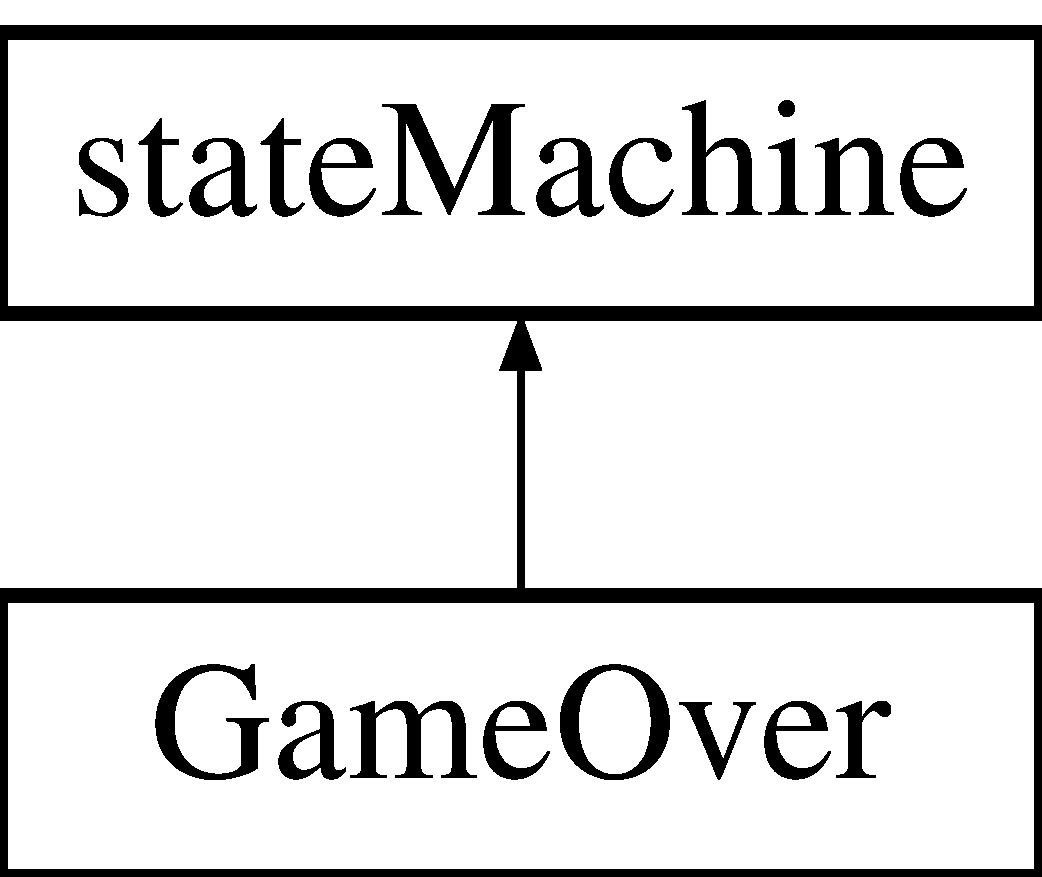
\includegraphics[height=2.000000cm]{class_game_over}
\end{center}
\end{figure}
\subsection*{Public Member Functions}
\begin{DoxyCompactItemize}
\item 
\hyperlink{class_game_over_a0ff11ac73026d574c5b393e825f10a1b}{Game\-Over} ()
\item 
\hyperlink{class_game_over_ae36951a153d25d52fab7cbc7a85bbbbd}{$\sim$\-Game\-Over} ()
\item 
void \hyperlink{class_game_over_ac983ca4c0d92982da2f27a1a3758d91e}{handle\-\_\-events} ()
\item 
void \hyperlink{class_game_over_a4ff51266107ff11b3b10a2e0187eb3f6}{logic} ()
\begin{DoxyCompactList}\small\item\em Handle events for every state. \end{DoxyCompactList}\item 
void \hyperlink{class_game_over_acaf9a4bea8b0e3e051d58b9ff4c80bec}{render} ()
\begin{DoxyCompactList}\small\item\em Handle Logic for each state. \end{DoxyCompactList}\end{DoxyCompactItemize}


\subsection{Constructor \& Destructor Documentation}
\hypertarget{class_game_over_a0ff11ac73026d574c5b393e825f10a1b}{\index{Game\-Over@{Game\-Over}!Game\-Over@{Game\-Over}}
\index{Game\-Over@{Game\-Over}!GameOver@{Game\-Over}}
\subsubsection[{Game\-Over}]{\setlength{\rightskip}{0pt plus 5cm}Game\-Over\-::\-Game\-Over (
\begin{DoxyParamCaption}
{}
\end{DoxyParamCaption}
)}}\label{class_game_over_a0ff11ac73026d574c5b393e825f10a1b}
\hypertarget{class_game_over_ae36951a153d25d52fab7cbc7a85bbbbd}{\index{Game\-Over@{Game\-Over}!$\sim$\-Game\-Over@{$\sim$\-Game\-Over}}
\index{$\sim$\-Game\-Over@{$\sim$\-Game\-Over}!GameOver@{Game\-Over}}
\subsubsection[{$\sim$\-Game\-Over}]{\setlength{\rightskip}{0pt plus 5cm}Game\-Over\-::$\sim$\-Game\-Over (
\begin{DoxyParamCaption}
{}
\end{DoxyParamCaption}
)}}\label{class_game_over_ae36951a153d25d52fab7cbc7a85bbbbd}


\subsection{Member Function Documentation}
\hypertarget{class_game_over_ac983ca4c0d92982da2f27a1a3758d91e}{\index{Game\-Over@{Game\-Over}!handle\-\_\-events@{handle\-\_\-events}}
\index{handle\-\_\-events@{handle\-\_\-events}!GameOver@{Game\-Over}}
\subsubsection[{handle\-\_\-events}]{\setlength{\rightskip}{0pt plus 5cm}void Game\-Over\-::handle\-\_\-events (
\begin{DoxyParamCaption}
{}
\end{DoxyParamCaption}
)\hspace{0.3cm}{\ttfamily [virtual]}}}\label{class_game_over_ac983ca4c0d92982da2f27a1a3758d91e}


Reimplemented from \hyperlink{classstate_machine_a3fb12b413428098b6e98c0c1525db375}{state\-Machine}.

\hypertarget{class_game_over_a4ff51266107ff11b3b10a2e0187eb3f6}{\index{Game\-Over@{Game\-Over}!logic@{logic}}
\index{logic@{logic}!GameOver@{Game\-Over}}
\subsubsection[{logic}]{\setlength{\rightskip}{0pt plus 5cm}void Game\-Over\-::logic (
\begin{DoxyParamCaption}
{}
\end{DoxyParamCaption}
)\hspace{0.3cm}{\ttfamily [virtual]}}}\label{class_game_over_a4ff51266107ff11b3b10a2e0187eb3f6}


Handle events for every state. 



Reimplemented from \hyperlink{classstate_machine_a3823bf8d9d05334eccc5d1d62a099714}{state\-Machine}.

\hypertarget{class_game_over_acaf9a4bea8b0e3e051d58b9ff4c80bec}{\index{Game\-Over@{Game\-Over}!render@{render}}
\index{render@{render}!GameOver@{Game\-Over}}
\subsubsection[{render}]{\setlength{\rightskip}{0pt plus 5cm}void Game\-Over\-::render (
\begin{DoxyParamCaption}
{}
\end{DoxyParamCaption}
)\hspace{0.3cm}{\ttfamily [virtual]}}}\label{class_game_over_acaf9a4bea8b0e3e051d58b9ff4c80bec}


Handle Logic for each state. 



Reimplemented from \hyperlink{classstate_machine_adf943abf2ca060aa80746f2cdec4daf0}{state\-Machine}.



The documentation for this class was generated from the following file\-:\begin{DoxyCompactItemize}
\item 
/home/ludkiller/projects/\-Super\-Guy/src/\-State\-Machine/\hyperlink{_state_machine_8h}{State\-Machine.\-h}\end{DoxyCompactItemize}

\hypertarget{class_intro}{\section{Intro Class Reference}
\label{class_intro}\index{Intro@{Intro}}
}


{\ttfamily \#include $<$State\-Machine.\-h$>$}

Inheritance diagram for Intro\-:\begin{figure}[H]
\begin{center}
\leavevmode
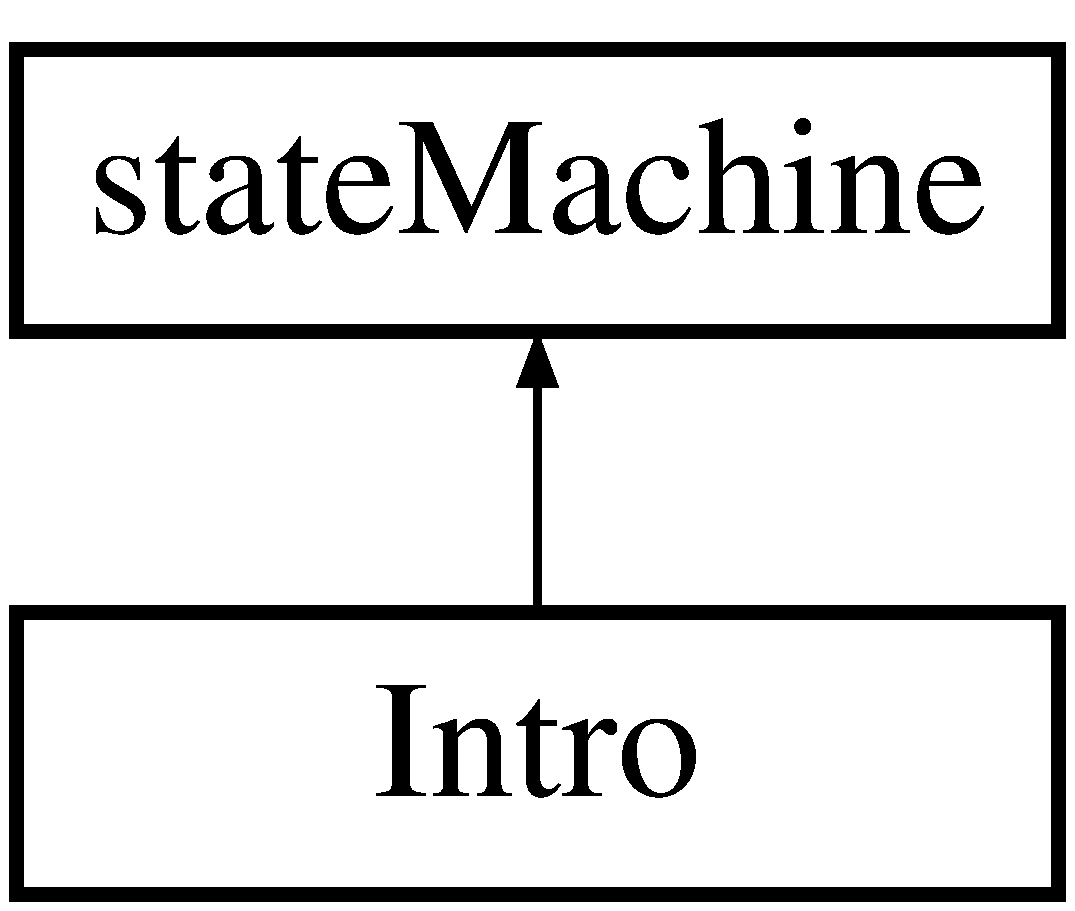
\includegraphics[height=2.000000cm]{class_intro}
\end{center}
\end{figure}
\subsection*{Public Member Functions}
\begin{DoxyCompactItemize}
\item 
\hyperlink{class_intro_a39875a338e68b4e2fba74693131ae498}{Intro} ()
\item 
\hyperlink{class_intro_a024067dadaf97daca3bfeb0f22e9c183}{$\sim$\-Intro} ()
\item 
void \hyperlink{class_intro_ab559f39689d24f41f3bc03791241974f}{handle\-\_\-events} ()
\item 
void \hyperlink{class_intro_abca960766a7e6e977be5e56e59637afd}{logic} ()
\begin{DoxyCompactList}\small\item\em Handle events for every state. \end{DoxyCompactList}\item 
void \hyperlink{class_intro_afa2ad2d82a78c9fbc38c1fdeeae80992}{render} ()
\begin{DoxyCompactList}\small\item\em Handle Logic for each state. \end{DoxyCompactList}\end{DoxyCompactItemize}


\subsection{Constructor \& Destructor Documentation}
\hypertarget{class_intro_a39875a338e68b4e2fba74693131ae498}{\index{Intro@{Intro}!Intro@{Intro}}
\index{Intro@{Intro}!Intro@{Intro}}
\subsubsection[{Intro}]{\setlength{\rightskip}{0pt plus 5cm}Intro\-::\-Intro (
\begin{DoxyParamCaption}
{}
\end{DoxyParamCaption}
)}}\label{class_intro_a39875a338e68b4e2fba74693131ae498}
\hypertarget{class_intro_a024067dadaf97daca3bfeb0f22e9c183}{\index{Intro@{Intro}!$\sim$\-Intro@{$\sim$\-Intro}}
\index{$\sim$\-Intro@{$\sim$\-Intro}!Intro@{Intro}}
\subsubsection[{$\sim$\-Intro}]{\setlength{\rightskip}{0pt plus 5cm}Intro\-::$\sim$\-Intro (
\begin{DoxyParamCaption}
{}
\end{DoxyParamCaption}
)}}\label{class_intro_a024067dadaf97daca3bfeb0f22e9c183}


\subsection{Member Function Documentation}
\hypertarget{class_intro_ab559f39689d24f41f3bc03791241974f}{\index{Intro@{Intro}!handle\-\_\-events@{handle\-\_\-events}}
\index{handle\-\_\-events@{handle\-\_\-events}!Intro@{Intro}}
\subsubsection[{handle\-\_\-events}]{\setlength{\rightskip}{0pt plus 5cm}void Intro\-::handle\-\_\-events (
\begin{DoxyParamCaption}
{}
\end{DoxyParamCaption}
)\hspace{0.3cm}{\ttfamily [virtual]}}}\label{class_intro_ab559f39689d24f41f3bc03791241974f}


Reimplemented from \hyperlink{classstate_machine_a3fb12b413428098b6e98c0c1525db375}{state\-Machine}.

\hypertarget{class_intro_abca960766a7e6e977be5e56e59637afd}{\index{Intro@{Intro}!logic@{logic}}
\index{logic@{logic}!Intro@{Intro}}
\subsubsection[{logic}]{\setlength{\rightskip}{0pt plus 5cm}void Intro\-::logic (
\begin{DoxyParamCaption}
{}
\end{DoxyParamCaption}
)\hspace{0.3cm}{\ttfamily [virtual]}}}\label{class_intro_abca960766a7e6e977be5e56e59637afd}


Handle events for every state. 



Reimplemented from \hyperlink{classstate_machine_a3823bf8d9d05334eccc5d1d62a099714}{state\-Machine}.

\hypertarget{class_intro_afa2ad2d82a78c9fbc38c1fdeeae80992}{\index{Intro@{Intro}!render@{render}}
\index{render@{render}!Intro@{Intro}}
\subsubsection[{render}]{\setlength{\rightskip}{0pt plus 5cm}void Intro\-::render (
\begin{DoxyParamCaption}
{}
\end{DoxyParamCaption}
)\hspace{0.3cm}{\ttfamily [virtual]}}}\label{class_intro_afa2ad2d82a78c9fbc38c1fdeeae80992}


Handle Logic for each state. 



Reimplemented from \hyperlink{classstate_machine_adf943abf2ca060aa80746f2cdec4daf0}{state\-Machine}.



The documentation for this class was generated from the following file\-:\begin{DoxyCompactItemize}
\item 
/home/ludkiller/projects/\-Super\-Guy/src/\-State\-Machine/\hyperlink{_state_machine_8h}{State\-Machine.\-h}\end{DoxyCompactItemize}

\hypertarget{classlog}{\section{log Class Reference}
\label{classlog}\index{log@{log}}
}


{\ttfamily \#include $<$log.\-h$>$}

\subsection*{Public Member Functions}
\begin{DoxyCompactItemize}
\item 
\hyperlink{classlog_a974f291f7491c11128b701aaf95a7cc2}{log} ()
\item 
\hyperlink{classlog_a4742c7f6ebc53ddf0caf9ac43402175b}{$\sim$log} ()
\end{DoxyCompactItemize}
\subsection*{Static Public Member Functions}
\begin{DoxyCompactItemize}
\item 
static bool \hyperlink{classlog_ab0d99a8357cae3f0b5dfa3435b2a4fc1}{open} (const char $\ast$file)
\item 
static void \hyperlink{classlog_add1b87f0d0d4b68af52eaf9b2d26c4f6}{close} ()
\item 
static void \hyperlink{classlog_a505d87de8e6f35082a66df3c766b968f}{info} (const char $\ast$msg,...)
\item 
static void \hyperlink{classlog_ada241500acc3729078a19b649889eaf7}{error} (const char $\ast$msg,...)
\item 
static void \hyperlink{classlog_a4a8d2825194c68a9966fa36f75d14942}{warning} (const char $\ast$msg,...)
\end{DoxyCompactItemize}


\subsection{Constructor \& Destructor Documentation}
\hypertarget{classlog_a974f291f7491c11128b701aaf95a7cc2}{\index{log@{log}!log@{log}}
\index{log@{log}!log@{log}}
\subsubsection[{log}]{\setlength{\rightskip}{0pt plus 5cm}log\-::log (
\begin{DoxyParamCaption}
{}
\end{DoxyParamCaption}
)}}\label{classlog_a974f291f7491c11128b701aaf95a7cc2}
\hypertarget{classlog_a4742c7f6ebc53ddf0caf9ac43402175b}{\index{log@{log}!$\sim$log@{$\sim$log}}
\index{$\sim$log@{$\sim$log}!log@{log}}
\subsubsection[{$\sim$log}]{\setlength{\rightskip}{0pt plus 5cm}log\-::$\sim$log (
\begin{DoxyParamCaption}
{}
\end{DoxyParamCaption}
)}}\label{classlog_a4742c7f6ebc53ddf0caf9ac43402175b}


\subsection{Member Function Documentation}
\hypertarget{classlog_add1b87f0d0d4b68af52eaf9b2d26c4f6}{\index{log@{log}!close@{close}}
\index{close@{close}!log@{log}}
\subsubsection[{close}]{\setlength{\rightskip}{0pt plus 5cm}void log\-::close (
\begin{DoxyParamCaption}
{}
\end{DoxyParamCaption}
)\hspace{0.3cm}{\ttfamily [static]}}}\label{classlog_add1b87f0d0d4b68af52eaf9b2d26c4f6}
\hypertarget{classlog_ada241500acc3729078a19b649889eaf7}{\index{log@{log}!error@{error}}
\index{error@{error}!log@{log}}
\subsubsection[{error}]{\setlength{\rightskip}{0pt plus 5cm}void log\-::error (
\begin{DoxyParamCaption}
\item[{const char $\ast$}]{msg, }
\item[{}]{...}
\end{DoxyParamCaption}
)\hspace{0.3cm}{\ttfamily [static]}}}\label{classlog_ada241500acc3729078a19b649889eaf7}
\hypertarget{classlog_a505d87de8e6f35082a66df3c766b968f}{\index{log@{log}!info@{info}}
\index{info@{info}!log@{log}}
\subsubsection[{info}]{\setlength{\rightskip}{0pt plus 5cm}void log\-::info (
\begin{DoxyParamCaption}
\item[{const char $\ast$}]{msg, }
\item[{}]{...}
\end{DoxyParamCaption}
)\hspace{0.3cm}{\ttfamily [static]}}}\label{classlog_a505d87de8e6f35082a66df3c766b968f}
\hypertarget{classlog_ab0d99a8357cae3f0b5dfa3435b2a4fc1}{\index{log@{log}!open@{open}}
\index{open@{open}!log@{log}}
\subsubsection[{open}]{\setlength{\rightskip}{0pt plus 5cm}bool log\-::open (
\begin{DoxyParamCaption}
\item[{const char $\ast$}]{file}
\end{DoxyParamCaption}
)\hspace{0.3cm}{\ttfamily [static]}}}\label{classlog_ab0d99a8357cae3f0b5dfa3435b2a4fc1}
\hypertarget{classlog_a4a8d2825194c68a9966fa36f75d14942}{\index{log@{log}!warning@{warning}}
\index{warning@{warning}!log@{log}}
\subsubsection[{warning}]{\setlength{\rightskip}{0pt plus 5cm}void log\-::warning (
\begin{DoxyParamCaption}
\item[{const char $\ast$}]{msg, }
\item[{}]{...}
\end{DoxyParamCaption}
)\hspace{0.3cm}{\ttfamily [static]}}}\label{classlog_a4a8d2825194c68a9966fa36f75d14942}


The documentation for this class was generated from the following files\-:\begin{DoxyCompactItemize}
\item 
/home/ludkiller/projects/\-Super\-Guy/src/\hyperlink{log_8h}{log.\-h}\item 
/home/ludkiller/projects/\-Super\-Guy/src/\hyperlink{log_8cpp}{log.\-cpp}\end{DoxyCompactItemize}

\hypertarget{class_stage1}{\section{Stage1 Class Reference}
\label{class_stage1}\index{Stage1@{Stage1}}
}


{\ttfamily \#include $<$State\-Machine.\-h$>$}

Inheritance diagram for Stage1\-:\begin{figure}[H]
\begin{center}
\leavevmode
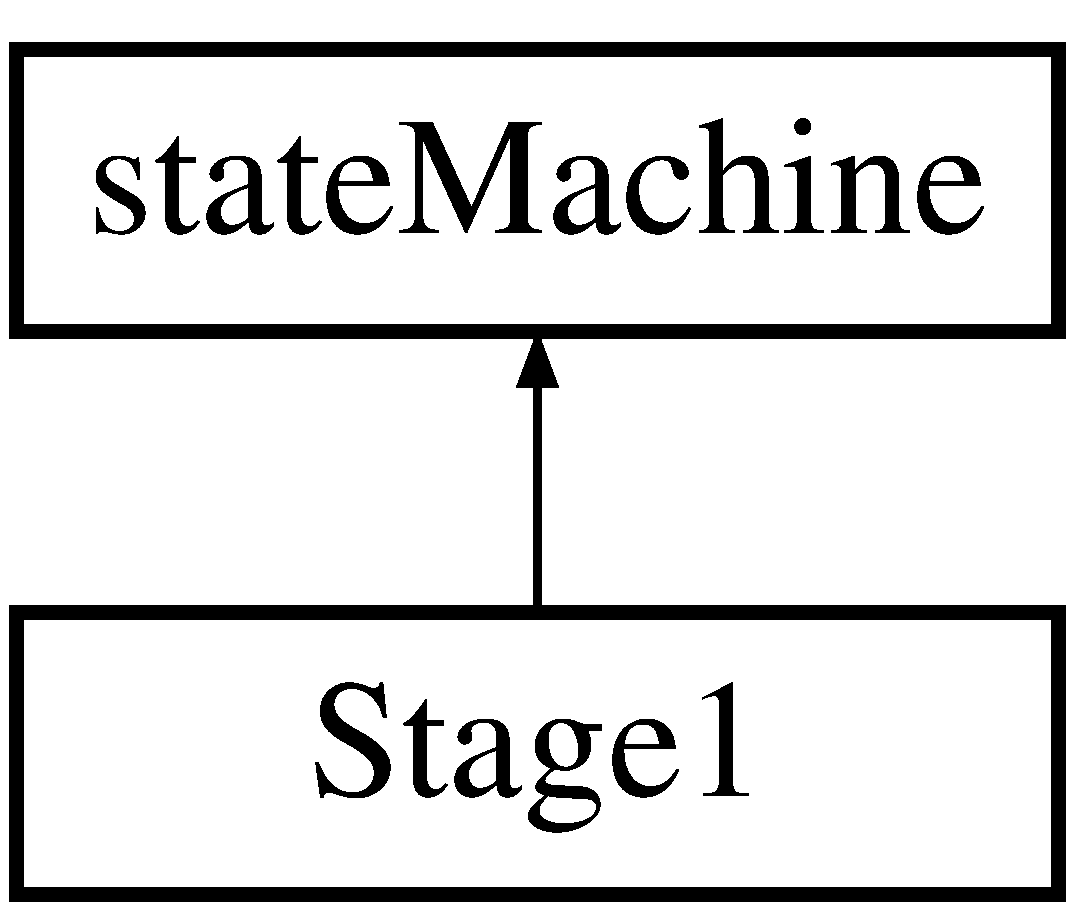
\includegraphics[height=2.000000cm]{class_stage1}
\end{center}
\end{figure}
\subsection*{Public Member Functions}
\begin{DoxyCompactItemize}
\item 
\hyperlink{class_stage1_a18240000454d844b1c183a203eddbf4b}{Stage1} ()
\begin{DoxyCompactList}\small\item\em Height Of \hyperlink{class_stage1}{Stage1}. \end{DoxyCompactList}\item 
\hyperlink{class_stage1_a0bd922af78678696112fe8d4091cfa4f}{$\sim$\-Stage1} ()
\begin{DoxyCompactList}\small\item\em Constructor for \hyperlink{class_stage1}{Stage1}. \end{DoxyCompactList}\item 
void \hyperlink{class_stage1_ae746fd19bf35b78535618cd5484d970c}{handle\-\_\-events} ()
\begin{DoxyCompactList}\small\item\em Destructor for \hyperlink{class_stage1}{Stage1}. \end{DoxyCompactList}\item 
void \hyperlink{class_stage1_ae7fe27770d40d654297f044e693af030}{logic} ()
\begin{DoxyCompactList}\small\item\em Handle \hyperlink{class_stage1}{Stage1} Events. \end{DoxyCompactList}\item 
void \hyperlink{class_stage1_a60be0ff24305d7d018219f985b5b9323}{render} ()
\begin{DoxyCompactList}\small\item\em Handle \hyperlink{class_stage1}{Stage1} Logic. \end{DoxyCompactList}\end{DoxyCompactItemize}


\subsection{Constructor \& Destructor Documentation}
\hypertarget{class_stage1_a18240000454d844b1c183a203eddbf4b}{\index{Stage1@{Stage1}!Stage1@{Stage1}}
\index{Stage1@{Stage1}!Stage1@{Stage1}}
\subsubsection[{Stage1}]{\setlength{\rightskip}{0pt plus 5cm}Stage1\-::\-Stage1 (
\begin{DoxyParamCaption}
{}
\end{DoxyParamCaption}
)}}\label{class_stage1_a18240000454d844b1c183a203eddbf4b}


Height Of \hyperlink{class_stage1}{Stage1}. 

\hypertarget{class_stage1_a0bd922af78678696112fe8d4091cfa4f}{\index{Stage1@{Stage1}!$\sim$\-Stage1@{$\sim$\-Stage1}}
\index{$\sim$\-Stage1@{$\sim$\-Stage1}!Stage1@{Stage1}}
\subsubsection[{$\sim$\-Stage1}]{\setlength{\rightskip}{0pt plus 5cm}Stage1\-::$\sim$\-Stage1 (
\begin{DoxyParamCaption}
{}
\end{DoxyParamCaption}
)}}\label{class_stage1_a0bd922af78678696112fe8d4091cfa4f}


Constructor for \hyperlink{class_stage1}{Stage1}. 



\subsection{Member Function Documentation}
\hypertarget{class_stage1_ae746fd19bf35b78535618cd5484d970c}{\index{Stage1@{Stage1}!handle\-\_\-events@{handle\-\_\-events}}
\index{handle\-\_\-events@{handle\-\_\-events}!Stage1@{Stage1}}
\subsubsection[{handle\-\_\-events}]{\setlength{\rightskip}{0pt plus 5cm}void Stage1\-::handle\-\_\-events (
\begin{DoxyParamCaption}
{}
\end{DoxyParamCaption}
)\hspace{0.3cm}{\ttfamily [virtual]}}}\label{class_stage1_ae746fd19bf35b78535618cd5484d970c}


Destructor for \hyperlink{class_stage1}{Stage1}. 



Reimplemented from \hyperlink{classstate_machine_a3fb12b413428098b6e98c0c1525db375}{state\-Machine}.

\hypertarget{class_stage1_ae7fe27770d40d654297f044e693af030}{\index{Stage1@{Stage1}!logic@{logic}}
\index{logic@{logic}!Stage1@{Stage1}}
\subsubsection[{logic}]{\setlength{\rightskip}{0pt plus 5cm}void Stage1\-::logic (
\begin{DoxyParamCaption}
{}
\end{DoxyParamCaption}
)\hspace{0.3cm}{\ttfamily [virtual]}}}\label{class_stage1_ae7fe27770d40d654297f044e693af030}


Handle \hyperlink{class_stage1}{Stage1} Events. 



Reimplemented from \hyperlink{classstate_machine_a3823bf8d9d05334eccc5d1d62a099714}{state\-Machine}.

\hypertarget{class_stage1_a60be0ff24305d7d018219f985b5b9323}{\index{Stage1@{Stage1}!render@{render}}
\index{render@{render}!Stage1@{Stage1}}
\subsubsection[{render}]{\setlength{\rightskip}{0pt plus 5cm}void Stage1\-::render (
\begin{DoxyParamCaption}
{}
\end{DoxyParamCaption}
)\hspace{0.3cm}{\ttfamily [virtual]}}}\label{class_stage1_a60be0ff24305d7d018219f985b5b9323}


Handle \hyperlink{class_stage1}{Stage1} Logic. 



Reimplemented from \hyperlink{classstate_machine_adf943abf2ca060aa80746f2cdec4daf0}{state\-Machine}.



The documentation for this class was generated from the following files\-:\begin{DoxyCompactItemize}
\item 
/home/ludkiller/projects/\-Super\-Guy/src/\-State\-Machine/\hyperlink{_state_machine_8h}{State\-Machine.\-h}\item 
/home/ludkiller/projects/\-Super\-Guy/src/\-State\-Machine/\hyperlink{_state_machine_8cpp}{State\-Machine.\-cpp}\end{DoxyCompactItemize}

\hypertarget{classstate_machine}{\section{state\-Machine Class Reference}
\label{classstate_machine}\index{state\-Machine@{state\-Machine}}
}


States for State Machine.  




{\ttfamily \#include $<$State\-Machine.\-h$>$}

Inheritance diagram for state\-Machine\-:\begin{figure}[H]
\begin{center}
\leavevmode
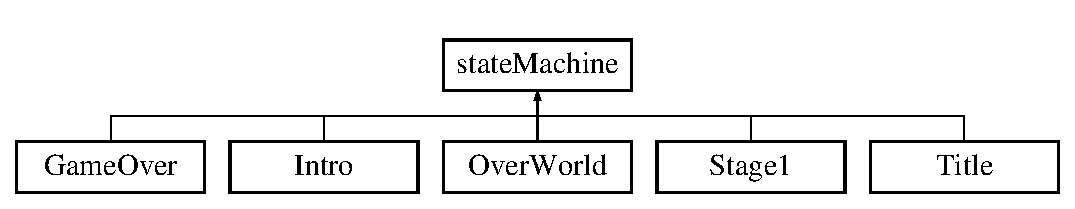
\includegraphics[height=2.000000cm]{classstate_machine}
\end{center}
\end{figure}
\subsection*{Public Member Functions}
\begin{DoxyCompactItemize}
\item 
virtual void \hyperlink{classstate_machine_a3fb12b413428098b6e98c0c1525db375}{handle\-\_\-events} ()
\item 
virtual void \hyperlink{classstate_machine_a3823bf8d9d05334eccc5d1d62a099714}{logic} ()
\begin{DoxyCompactList}\small\item\em Handle events for every state. \end{DoxyCompactList}\item 
virtual void \hyperlink{classstate_machine_adf943abf2ca060aa80746f2cdec4daf0}{render} ()
\begin{DoxyCompactList}\small\item\em Handle Logic for each state. \end{DoxyCompactList}\item 
virtual \hyperlink{classstate_machine_afca4850a1876eed86643aed4cc529dc7}{$\sim$state\-Machine} ()
\begin{DoxyCompactList}\small\item\em Handle rendering for each state. \end{DoxyCompactList}\item 
void \hyperlink{classstate_machine_aa37b1c8ff364025c2a1f82d92f9a1ce0}{set\-Next\-State} ()
\begin{DoxyCompactList}\small\item\em Destructor for each state. \end{DoxyCompactList}\item 
void \hyperlink{classstate_machine_a81432eab64611f3d7ac5338aee324257}{change\-State} ()
\begin{DoxyCompactList}\small\item\em Sets our next state. \end{DoxyCompactList}\end{DoxyCompactItemize}


\subsection{Detailed Description}
States for State Machine. 

\subsection{Constructor \& Destructor Documentation}
\hypertarget{classstate_machine_afca4850a1876eed86643aed4cc529dc7}{\index{state\-Machine@{state\-Machine}!$\sim$state\-Machine@{$\sim$state\-Machine}}
\index{$\sim$state\-Machine@{$\sim$state\-Machine}!stateMachine@{state\-Machine}}
\subsubsection[{$\sim$state\-Machine}]{\setlength{\rightskip}{0pt plus 5cm}virtual state\-Machine\-::$\sim$state\-Machine (
\begin{DoxyParamCaption}
{}
\end{DoxyParamCaption}
)\hspace{0.3cm}{\ttfamily [virtual]}}}\label{classstate_machine_afca4850a1876eed86643aed4cc529dc7}


Handle rendering for each state. 



\subsection{Member Function Documentation}
\hypertarget{classstate_machine_a81432eab64611f3d7ac5338aee324257}{\index{state\-Machine@{state\-Machine}!change\-State@{change\-State}}
\index{change\-State@{change\-State}!stateMachine@{state\-Machine}}
\subsubsection[{change\-State}]{\setlength{\rightskip}{0pt plus 5cm}void state\-Machine\-::change\-State (
\begin{DoxyParamCaption}
{}
\end{DoxyParamCaption}
)}}\label{classstate_machine_a81432eab64611f3d7ac5338aee324257}


Sets our next state. 

\hypertarget{classstate_machine_a3fb12b413428098b6e98c0c1525db375}{\index{state\-Machine@{state\-Machine}!handle\-\_\-events@{handle\-\_\-events}}
\index{handle\-\_\-events@{handle\-\_\-events}!stateMachine@{state\-Machine}}
\subsubsection[{handle\-\_\-events}]{\setlength{\rightskip}{0pt plus 5cm}virtual void state\-Machine\-::handle\-\_\-events (
\begin{DoxyParamCaption}
{}
\end{DoxyParamCaption}
)\hspace{0.3cm}{\ttfamily [virtual]}}}\label{classstate_machine_a3fb12b413428098b6e98c0c1525db375}


Reimplemented in \hyperlink{class_game_over_ac983ca4c0d92982da2f27a1a3758d91e}{Game\-Over}, \hyperlink{class_stage1_ae746fd19bf35b78535618cd5484d970c}{Stage1}, \hyperlink{class_title_a679fe0df9fda9088027619dc1bed3780}{Title}, and \hyperlink{class_intro_ab559f39689d24f41f3bc03791241974f}{Intro}.

\hypertarget{classstate_machine_a3823bf8d9d05334eccc5d1d62a099714}{\index{state\-Machine@{state\-Machine}!logic@{logic}}
\index{logic@{logic}!stateMachine@{state\-Machine}}
\subsubsection[{logic}]{\setlength{\rightskip}{0pt plus 5cm}virtual void state\-Machine\-::logic (
\begin{DoxyParamCaption}
{}
\end{DoxyParamCaption}
)\hspace{0.3cm}{\ttfamily [virtual]}}}\label{classstate_machine_a3823bf8d9d05334eccc5d1d62a099714}


Handle events for every state. 



Reimplemented in \hyperlink{class_game_over_a4ff51266107ff11b3b10a2e0187eb3f6}{Game\-Over}, \hyperlink{class_stage1_ae7fe27770d40d654297f044e693af030}{Stage1}, \hyperlink{class_title_a530e17f16f634a0385a8d37ed6a57104}{Title}, and \hyperlink{class_intro_abca960766a7e6e977be5e56e59637afd}{Intro}.

\hypertarget{classstate_machine_adf943abf2ca060aa80746f2cdec4daf0}{\index{state\-Machine@{state\-Machine}!render@{render}}
\index{render@{render}!stateMachine@{state\-Machine}}
\subsubsection[{render}]{\setlength{\rightskip}{0pt plus 5cm}virtual void state\-Machine\-::render (
\begin{DoxyParamCaption}
{}
\end{DoxyParamCaption}
)\hspace{0.3cm}{\ttfamily [virtual]}}}\label{classstate_machine_adf943abf2ca060aa80746f2cdec4daf0}


Handle Logic for each state. 



Reimplemented in \hyperlink{class_game_over_acaf9a4bea8b0e3e051d58b9ff4c80bec}{Game\-Over}, \hyperlink{class_stage1_a60be0ff24305d7d018219f985b5b9323}{Stage1}, \hyperlink{class_title_a4a9fe899fdb92d6d82bbb88b949cdeaf}{Title}, and \hyperlink{class_intro_afa2ad2d82a78c9fbc38c1fdeeae80992}{Intro}.

\hypertarget{classstate_machine_aa37b1c8ff364025c2a1f82d92f9a1ce0}{\index{state\-Machine@{state\-Machine}!set\-Next\-State@{set\-Next\-State}}
\index{set\-Next\-State@{set\-Next\-State}!stateMachine@{state\-Machine}}
\subsubsection[{set\-Next\-State}]{\setlength{\rightskip}{0pt plus 5cm}void state\-Machine\-::set\-Next\-State (
\begin{DoxyParamCaption}
{}
\end{DoxyParamCaption}
)}}\label{classstate_machine_aa37b1c8ff364025c2a1f82d92f9a1ce0}


Destructor for each state. 



The documentation for this class was generated from the following file\-:\begin{DoxyCompactItemize}
\item 
/home/ludkiller/projects/\-Super\-Guy/src/\-State\-Machine/\hyperlink{_state_machine_8h}{State\-Machine.\-h}\end{DoxyCompactItemize}

\hypertarget{classtexture}{\section{texture Class Reference}
\label{classtexture}\index{texture@{texture}}
}


{\ttfamily \#include $<$texture.\-h$>$}

\subsection*{Public Member Functions}
\begin{DoxyCompactItemize}
\item 
\hyperlink{classtexture_a8dd00d9a5b53b82421efd40d1471f877}{texture} (const char $\ast$file, int count)
\item 
\hyperlink{classtexture_a612f21e2f69df18b54a56ade8e4eec59}{texture} (S\-D\-L\-\_\-\-Surface $\ast$tex)
\item 
\hyperlink{classtexture_a5b4f688537fcc04427d7aaf2a35996bd}{$\sim$texture} ()
\item 
\hyperlink{classtexture}{texture} $\ast$ \hyperlink{classtexture_ab5a6671d4f348d5e62eedd2c4519c5dd}{get\-Texture\-At\-Pos} (int pos)
\item 
S\-D\-L\-\_\-\-Surface $\ast$ \hyperlink{classtexture_ac5ee5635e548e3939f79fd6e596221d3}{get\-Texture} ()
\end{DoxyCompactItemize}


\subsection{Constructor \& Destructor Documentation}
\hypertarget{classtexture_a8dd00d9a5b53b82421efd40d1471f877}{\index{texture@{texture}!texture@{texture}}
\index{texture@{texture}!texture@{texture}}
\subsubsection[{texture}]{\setlength{\rightskip}{0pt plus 5cm}texture\-::texture (
\begin{DoxyParamCaption}
\item[{const char $\ast$}]{file, }
\item[{int}]{count}
\end{DoxyParamCaption}
)}}\label{classtexture_a8dd00d9a5b53b82421efd40d1471f877}
\hypertarget{classtexture_a612f21e2f69df18b54a56ade8e4eec59}{\index{texture@{texture}!texture@{texture}}
\index{texture@{texture}!texture@{texture}}
\subsubsection[{texture}]{\setlength{\rightskip}{0pt plus 5cm}texture\-::texture (
\begin{DoxyParamCaption}
\item[{S\-D\-L\-\_\-\-Surface $\ast$}]{tex}
\end{DoxyParamCaption}
)}}\label{classtexture_a612f21e2f69df18b54a56ade8e4eec59}
\hypertarget{classtexture_a5b4f688537fcc04427d7aaf2a35996bd}{\index{texture@{texture}!$\sim$texture@{$\sim$texture}}
\index{$\sim$texture@{$\sim$texture}!texture@{texture}}
\subsubsection[{$\sim$texture}]{\setlength{\rightskip}{0pt plus 5cm}texture\-::$\sim$texture (
\begin{DoxyParamCaption}
{}
\end{DoxyParamCaption}
)}}\label{classtexture_a5b4f688537fcc04427d7aaf2a35996bd}


\subsection{Member Function Documentation}
\hypertarget{classtexture_ac5ee5635e548e3939f79fd6e596221d3}{\index{texture@{texture}!get\-Texture@{get\-Texture}}
\index{get\-Texture@{get\-Texture}!texture@{texture}}
\subsubsection[{get\-Texture}]{\setlength{\rightskip}{0pt plus 5cm}S\-D\-L\-\_\-\-Surface $\ast$ texture\-::get\-Texture (
\begin{DoxyParamCaption}
{}
\end{DoxyParamCaption}
)}}\label{classtexture_ac5ee5635e548e3939f79fd6e596221d3}
\hypertarget{classtexture_ab5a6671d4f348d5e62eedd2c4519c5dd}{\index{texture@{texture}!get\-Texture\-At\-Pos@{get\-Texture\-At\-Pos}}
\index{get\-Texture\-At\-Pos@{get\-Texture\-At\-Pos}!texture@{texture}}
\subsubsection[{get\-Texture\-At\-Pos}]{\setlength{\rightskip}{0pt plus 5cm}{\bf texture} $\ast$ texture\-::get\-Texture\-At\-Pos (
\begin{DoxyParamCaption}
\item[{int}]{pos}
\end{DoxyParamCaption}
)}}\label{classtexture_ab5a6671d4f348d5e62eedd2c4519c5dd}


The documentation for this class was generated from the following files\-:\begin{DoxyCompactItemize}
\item 
/home/ludkiller/projects/\-Super\-Guy/src/engine/\hyperlink{texture_8h}{texture.\-h}\item 
/home/ludkiller/projects/\-Super\-Guy/src/engine/\hyperlink{texture_8cpp}{texture.\-cpp}\end{DoxyCompactItemize}

\hypertarget{class_title}{\section{Title Class Reference}
\label{class_title}\index{Title@{Title}}
}


{\ttfamily \#include $<$State\-Machine.\-h$>$}

Inheritance diagram for Title\-:\begin{figure}[H]
\begin{center}
\leavevmode
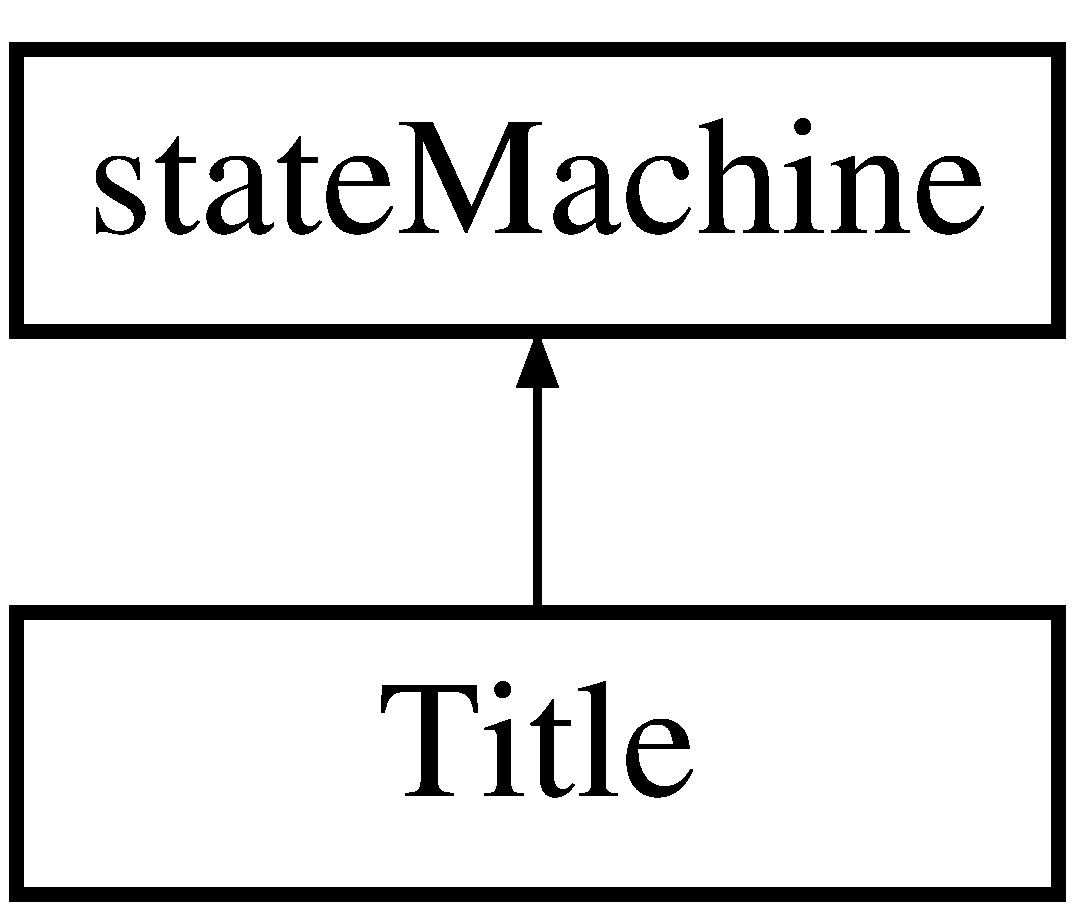
\includegraphics[height=2.000000cm]{class_title}
\end{center}
\end{figure}
\subsection*{Public Member Functions}
\begin{DoxyCompactItemize}
\item 
\hyperlink{class_title_a56ca0b368a213295649d75c62577e4bb}{Title} ()
\item 
\hyperlink{class_title_aa0423651e6010e406b1c1052724b785c}{$\sim$\-Title} ()
\item 
void \hyperlink{class_title_a679fe0df9fda9088027619dc1bed3780}{handle\-\_\-events} ()
\item 
void \hyperlink{class_title_a530e17f16f634a0385a8d37ed6a57104}{logic} ()
\begin{DoxyCompactList}\small\item\em Handle events for every state. \end{DoxyCompactList}\item 
void \hyperlink{class_title_a4a9fe899fdb92d6d82bbb88b949cdeaf}{render} ()
\begin{DoxyCompactList}\small\item\em Handle Logic for each state. \end{DoxyCompactList}\end{DoxyCompactItemize}


\subsection{Constructor \& Destructor Documentation}
\hypertarget{class_title_a56ca0b368a213295649d75c62577e4bb}{\index{Title@{Title}!Title@{Title}}
\index{Title@{Title}!Title@{Title}}
\subsubsection[{Title}]{\setlength{\rightskip}{0pt plus 5cm}Title\-::\-Title (
\begin{DoxyParamCaption}
{}
\end{DoxyParamCaption}
)}}\label{class_title_a56ca0b368a213295649d75c62577e4bb}
\hypertarget{class_title_aa0423651e6010e406b1c1052724b785c}{\index{Title@{Title}!$\sim$\-Title@{$\sim$\-Title}}
\index{$\sim$\-Title@{$\sim$\-Title}!Title@{Title}}
\subsubsection[{$\sim$\-Title}]{\setlength{\rightskip}{0pt plus 5cm}Title\-::$\sim$\-Title (
\begin{DoxyParamCaption}
{}
\end{DoxyParamCaption}
)}}\label{class_title_aa0423651e6010e406b1c1052724b785c}


\subsection{Member Function Documentation}
\hypertarget{class_title_a679fe0df9fda9088027619dc1bed3780}{\index{Title@{Title}!handle\-\_\-events@{handle\-\_\-events}}
\index{handle\-\_\-events@{handle\-\_\-events}!Title@{Title}}
\subsubsection[{handle\-\_\-events}]{\setlength{\rightskip}{0pt plus 5cm}void Title\-::handle\-\_\-events (
\begin{DoxyParamCaption}
{}
\end{DoxyParamCaption}
)\hspace{0.3cm}{\ttfamily [virtual]}}}\label{class_title_a679fe0df9fda9088027619dc1bed3780}


Reimplemented from \hyperlink{classstate_machine_a3fb12b413428098b6e98c0c1525db375}{state\-Machine}.

\hypertarget{class_title_a530e17f16f634a0385a8d37ed6a57104}{\index{Title@{Title}!logic@{logic}}
\index{logic@{logic}!Title@{Title}}
\subsubsection[{logic}]{\setlength{\rightskip}{0pt plus 5cm}void Title\-::logic (
\begin{DoxyParamCaption}
{}
\end{DoxyParamCaption}
)\hspace{0.3cm}{\ttfamily [virtual]}}}\label{class_title_a530e17f16f634a0385a8d37ed6a57104}


Handle events for every state. 



Reimplemented from \hyperlink{classstate_machine_a3823bf8d9d05334eccc5d1d62a099714}{state\-Machine}.

\hypertarget{class_title_a4a9fe899fdb92d6d82bbb88b949cdeaf}{\index{Title@{Title}!render@{render}}
\index{render@{render}!Title@{Title}}
\subsubsection[{render}]{\setlength{\rightskip}{0pt plus 5cm}void Title\-::render (
\begin{DoxyParamCaption}
{}
\end{DoxyParamCaption}
)\hspace{0.3cm}{\ttfamily [virtual]}}}\label{class_title_a4a9fe899fdb92d6d82bbb88b949cdeaf}


Handle Logic for each state. 



Reimplemented from \hyperlink{classstate_machine_adf943abf2ca060aa80746f2cdec4daf0}{state\-Machine}.



The documentation for this class was generated from the following file\-:\begin{DoxyCompactItemize}
\item 
/home/ludkiller/projects/\-Super\-Guy/src/\-State\-Machine/\hyperlink{_state_machine_8h}{State\-Machine.\-h}\end{DoxyCompactItemize}

\chapter{File Documentation}
\hypertarget{_a_i_entity_8cpp}{\section{/home/ludkiller/projects/\-Super\-Guy/src/enemy/\-A\-I\-Entity.cpp File Reference}
\label{_a_i_entity_8cpp}\index{/home/ludkiller/projects/\-Super\-Guy/src/enemy/\-A\-I\-Entity.\-cpp@{/home/ludkiller/projects/\-Super\-Guy/src/enemy/\-A\-I\-Entity.\-cpp}}
}

\hypertarget{_a_i_entity_8h}{\section{/home/ludkiller/projects/\-Super\-Guy/src/enemy/\-A\-I\-Entity.h File Reference}
\label{_a_i_entity_8h}\index{/home/ludkiller/projects/\-Super\-Guy/src/enemy/\-A\-I\-Entity.\-h@{/home/ludkiller/projects/\-Super\-Guy/src/enemy/\-A\-I\-Entity.\-h}}
}

\hypertarget{enemy_ant_8cpp}{\section{/home/ludkiller/projects/\-Super\-Guy/src/enemy/enemy\-Ant.cpp File Reference}
\label{enemy_ant_8cpp}\index{/home/ludkiller/projects/\-Super\-Guy/src/enemy/enemy\-Ant.\-cpp@{/home/ludkiller/projects/\-Super\-Guy/src/enemy/enemy\-Ant.\-cpp}}
}
{\ttfamily \#include \char`\"{}enemy\-Ant.\-h\char`\"{}}\\*
{\ttfamily \#include $<$S\-D\-L2/\-S\-D\-L.\-h$>$}\\*

\hypertarget{enemy_ant_8h}{\section{/home/ludkiller/projects/\-Super\-Guy/src/enemy/enemy\-Ant.h File Reference}
\label{enemy_ant_8h}\index{/home/ludkiller/projects/\-Super\-Guy/src/enemy/enemy\-Ant.\-h@{/home/ludkiller/projects/\-Super\-Guy/src/enemy/enemy\-Ant.\-h}}
}
\subsection*{Classes}
\begin{DoxyCompactItemize}
\item 
class \hyperlink{classenemy_ant}{enemy\-Ant}
\end{DoxyCompactItemize}

\hypertarget{enemy_duck_8cpp}{\section{/home/ludkiller/projects/\-Super\-Guy/src/enemy/enemy\-Duck.cpp File Reference}
\label{enemy_duck_8cpp}\index{/home/ludkiller/projects/\-Super\-Guy/src/enemy/enemy\-Duck.\-cpp@{/home/ludkiller/projects/\-Super\-Guy/src/enemy/enemy\-Duck.\-cpp}}
}
{\ttfamily \#include \char`\"{}enemy\-Duck.\-h\char`\"{}}\\*
{\ttfamily \#include $<$S\-D\-L2/\-S\-D\-L.\-h$>$}\\*

\hypertarget{enemy_duck_8h}{\section{/home/ludkiller/projects/\-Super\-Guy/src/enemy/enemy\-Duck.h File Reference}
\label{enemy_duck_8h}\index{/home/ludkiller/projects/\-Super\-Guy/src/enemy/enemy\-Duck.\-h@{/home/ludkiller/projects/\-Super\-Guy/src/enemy/enemy\-Duck.\-h}}
}
\subsection*{Classes}
\begin{DoxyCompactItemize}
\item 
class \hyperlink{classenemy_duck}{enemy\-Duck}
\end{DoxyCompactItemize}

\hypertarget{dvar_8cpp}{\section{/home/ludkiller/projects/\-Super\-Guy/src/engine/dvar.cpp File Reference}
\label{dvar_8cpp}\index{/home/ludkiller/projects/\-Super\-Guy/src/engine/dvar.\-cpp@{/home/ludkiller/projects/\-Super\-Guy/src/engine/dvar.\-cpp}}
}
{\ttfamily \#include \char`\"{}dvar.\-h\char`\"{}}\\*
{\ttfamily \#include $<$cstdlib$>$}\\*

\hypertarget{dvar_8h}{\section{/home/ludkiller/projects/\-Super\-Guy/src/engine/dvar.h File Reference}
\label{dvar_8h}\index{/home/ludkiller/projects/\-Super\-Guy/src/engine/dvar.\-h@{/home/ludkiller/projects/\-Super\-Guy/src/engine/dvar.\-h}}
}
{\ttfamily \#include $<$stdint.\-h$>$}\\*
\subsection*{Classes}
\begin{DoxyCompactItemize}
\item 
union \hyperlink{uniondvar__value}{dvar\-\_\-value}
\item 
class \hyperlink{classdvar}{dvar}
\end{DoxyCompactItemize}
\subsection*{Typedefs}
\begin{DoxyCompactItemize}
\item 
typedef enum \hyperlink{dvar_8h_a8921c8a94863232fa751e940a4376072}{dvar\-\_\-flag} \hyperlink{dvar_8h_aefe39e0c960d504f76ed45445d970ee2}{dvar\-\_\-flag\-\_\-t}
\item 
typedef enum \hyperlink{dvar_8h_ad0c3c8845098903569009e434e197a38}{dvar\-\_\-type} \hyperlink{dvar_8h_a6a293e15d732e8bd2b0857ea14ebdaab}{dvar\-\_\-type\-\_\-t}
\item 
typedef union \hyperlink{uniondvar__value}{dvar\-\_\-value} \hyperlink{dvar_8h_a2dc7f3ad6d1f06950e9db0cc3813e0f7}{dvar\-\_\-value\-\_\-t}
\end{DoxyCompactItemize}
\subsection*{Enumerations}
\begin{DoxyCompactItemize}
\item 
enum \hyperlink{dvar_8h_a8921c8a94863232fa751e940a4376072}{dvar\-\_\-flag} \{ \hyperlink{dvar_8h_a8921c8a94863232fa751e940a4376072ae92c076b728effd4cfad58ecc2bc8206}{D\-V\-A\-R\-\_\-\-F\-L\-A\-G\-\_\-\-N\-O\-N\-E} =  0x00, 
\hyperlink{dvar_8h_a8921c8a94863232fa751e940a4376072abae57d7eb31e2671929f51d2abf43969}{D\-V\-A\-R\-\_\-\-F\-L\-A\-G\-\_\-\-S\-A\-V\-E} =  0x01, 
\hyperlink{dvar_8h_a8921c8a94863232fa751e940a4376072a70209570b2c12615658cc7b0a54fec0e}{D\-V\-A\-R\-\_\-\-F\-L\-A\-G\-\_\-\-R\-E\-A\-D\-O\-N\-L\-Y} =  0x02, 
\hyperlink{dvar_8h_a8921c8a94863232fa751e940a4376072ab1787e4c7ea90382bf5ece7bcb3e6827}{D\-V\-A\-R\-\_\-\-F\-L\-A\-G\-\_\-\-C\-H\-E\-A\-T} =  0x04
 \}
\item 
enum \hyperlink{dvar_8h_ad0c3c8845098903569009e434e197a38}{dvar\-\_\-type} \{ \hyperlink{dvar_8h_ad0c3c8845098903569009e434e197a38ad59bcd52e124814ec9574804b8858fd1}{D\-V\-A\-R\-\_\-\-T\-Y\-P\-E\-\_\-\-I\-N\-T}, 
\hyperlink{dvar_8h_ad0c3c8845098903569009e434e197a38a5cea3577a5e8ac57b13c3af0b12e2244}{D\-V\-A\-R\-\_\-\-T\-Y\-P\-E\-\_\-\-S\-T\-R\-I\-N\-G}, 
\hyperlink{dvar_8h_ad0c3c8845098903569009e434e197a38a071704830cbc99b5074254a1a1236f6c}{D\-V\-A\-R\-\_\-\-T\-Y\-P\-E\-\_\-\-D\-O\-U\-B\-L\-E}
 \}
\end{DoxyCompactItemize}


\subsection{Typedef Documentation}
\hypertarget{dvar_8h_aefe39e0c960d504f76ed45445d970ee2}{\index{dvar.\-h@{dvar.\-h}!dvar\-\_\-flag\-\_\-t@{dvar\-\_\-flag\-\_\-t}}
\index{dvar\-\_\-flag\-\_\-t@{dvar\-\_\-flag\-\_\-t}!dvar.h@{dvar.\-h}}
\subsubsection[{dvar\-\_\-flag\-\_\-t}]{\setlength{\rightskip}{0pt plus 5cm}typedef enum {\bf dvar\-\_\-flag}  {\bf dvar\-\_\-flag\-\_\-t}}}\label{dvar_8h_aefe39e0c960d504f76ed45445d970ee2}
\hypertarget{dvar_8h_a6a293e15d732e8bd2b0857ea14ebdaab}{\index{dvar.\-h@{dvar.\-h}!dvar\-\_\-type\-\_\-t@{dvar\-\_\-type\-\_\-t}}
\index{dvar\-\_\-type\-\_\-t@{dvar\-\_\-type\-\_\-t}!dvar.h@{dvar.\-h}}
\subsubsection[{dvar\-\_\-type\-\_\-t}]{\setlength{\rightskip}{0pt plus 5cm}typedef enum {\bf dvar\-\_\-type}  {\bf dvar\-\_\-type\-\_\-t}}}\label{dvar_8h_a6a293e15d732e8bd2b0857ea14ebdaab}
\hypertarget{dvar_8h_a2dc7f3ad6d1f06950e9db0cc3813e0f7}{\index{dvar.\-h@{dvar.\-h}!dvar\-\_\-value\-\_\-t@{dvar\-\_\-value\-\_\-t}}
\index{dvar\-\_\-value\-\_\-t@{dvar\-\_\-value\-\_\-t}!dvar.h@{dvar.\-h}}
\subsubsection[{dvar\-\_\-value\-\_\-t}]{\setlength{\rightskip}{0pt plus 5cm}typedef union {\bf dvar\-\_\-value}  {\bf dvar\-\_\-value\-\_\-t}}}\label{dvar_8h_a2dc7f3ad6d1f06950e9db0cc3813e0f7}


\subsection{Enumeration Type Documentation}
\hypertarget{dvar_8h_a8921c8a94863232fa751e940a4376072}{\index{dvar.\-h@{dvar.\-h}!dvar\-\_\-flag@{dvar\-\_\-flag}}
\index{dvar\-\_\-flag@{dvar\-\_\-flag}!dvar.h@{dvar.\-h}}
\subsubsection[{dvar\-\_\-flag}]{\setlength{\rightskip}{0pt plus 5cm}enum {\bf dvar\-\_\-flag}}}\label{dvar_8h_a8921c8a94863232fa751e940a4376072}
\begin{Desc}
\item[Enumerator\-: ]\par
\begin{description}
\index{D\-V\-A\-R\-\_\-\-F\-L\-A\-G\-\_\-\-N\-O\-N\-E@{D\-V\-A\-R\-\_\-\-F\-L\-A\-G\-\_\-\-N\-O\-N\-E}!dvar.\-h@{dvar.\-h}}\index{dvar.\-h@{dvar.\-h}!D\-V\-A\-R\-\_\-\-F\-L\-A\-G\-\_\-\-N\-O\-N\-E@{D\-V\-A\-R\-\_\-\-F\-L\-A\-G\-\_\-\-N\-O\-N\-E}}\item[{\em 
\hypertarget{dvar_8h_a8921c8a94863232fa751e940a4376072ae92c076b728effd4cfad58ecc2bc8206}{D\-V\-A\-R\-\_\-\-F\-L\-A\-G\-\_\-\-N\-O\-N\-E}\label{dvar_8h_a8921c8a94863232fa751e940a4376072ae92c076b728effd4cfad58ecc2bc8206}
}]\index{D\-V\-A\-R\-\_\-\-F\-L\-A\-G\-\_\-\-S\-A\-V\-E@{D\-V\-A\-R\-\_\-\-F\-L\-A\-G\-\_\-\-S\-A\-V\-E}!dvar.\-h@{dvar.\-h}}\index{dvar.\-h@{dvar.\-h}!D\-V\-A\-R\-\_\-\-F\-L\-A\-G\-\_\-\-S\-A\-V\-E@{D\-V\-A\-R\-\_\-\-F\-L\-A\-G\-\_\-\-S\-A\-V\-E}}\item[{\em 
\hypertarget{dvar_8h_a8921c8a94863232fa751e940a4376072abae57d7eb31e2671929f51d2abf43969}{D\-V\-A\-R\-\_\-\-F\-L\-A\-G\-\_\-\-S\-A\-V\-E}\label{dvar_8h_a8921c8a94863232fa751e940a4376072abae57d7eb31e2671929f51d2abf43969}
}]\index{D\-V\-A\-R\-\_\-\-F\-L\-A\-G\-\_\-\-R\-E\-A\-D\-O\-N\-L\-Y@{D\-V\-A\-R\-\_\-\-F\-L\-A\-G\-\_\-\-R\-E\-A\-D\-O\-N\-L\-Y}!dvar.\-h@{dvar.\-h}}\index{dvar.\-h@{dvar.\-h}!D\-V\-A\-R\-\_\-\-F\-L\-A\-G\-\_\-\-R\-E\-A\-D\-O\-N\-L\-Y@{D\-V\-A\-R\-\_\-\-F\-L\-A\-G\-\_\-\-R\-E\-A\-D\-O\-N\-L\-Y}}\item[{\em 
\hypertarget{dvar_8h_a8921c8a94863232fa751e940a4376072a70209570b2c12615658cc7b0a54fec0e}{D\-V\-A\-R\-\_\-\-F\-L\-A\-G\-\_\-\-R\-E\-A\-D\-O\-N\-L\-Y}\label{dvar_8h_a8921c8a94863232fa751e940a4376072a70209570b2c12615658cc7b0a54fec0e}
}]\index{D\-V\-A\-R\-\_\-\-F\-L\-A\-G\-\_\-\-C\-H\-E\-A\-T@{D\-V\-A\-R\-\_\-\-F\-L\-A\-G\-\_\-\-C\-H\-E\-A\-T}!dvar.\-h@{dvar.\-h}}\index{dvar.\-h@{dvar.\-h}!D\-V\-A\-R\-\_\-\-F\-L\-A\-G\-\_\-\-C\-H\-E\-A\-T@{D\-V\-A\-R\-\_\-\-F\-L\-A\-G\-\_\-\-C\-H\-E\-A\-T}}\item[{\em 
\hypertarget{dvar_8h_a8921c8a94863232fa751e940a4376072ab1787e4c7ea90382bf5ece7bcb3e6827}{D\-V\-A\-R\-\_\-\-F\-L\-A\-G\-\_\-\-C\-H\-E\-A\-T}\label{dvar_8h_a8921c8a94863232fa751e940a4376072ab1787e4c7ea90382bf5ece7bcb3e6827}
}]\end{description}
\end{Desc}

\hypertarget{dvar_8h_ad0c3c8845098903569009e434e197a38}{\index{dvar.\-h@{dvar.\-h}!dvar\-\_\-type@{dvar\-\_\-type}}
\index{dvar\-\_\-type@{dvar\-\_\-type}!dvar.h@{dvar.\-h}}
\subsubsection[{dvar\-\_\-type}]{\setlength{\rightskip}{0pt plus 5cm}enum {\bf dvar\-\_\-type}}}\label{dvar_8h_ad0c3c8845098903569009e434e197a38}
\begin{Desc}
\item[Enumerator\-: ]\par
\begin{description}
\index{D\-V\-A\-R\-\_\-\-T\-Y\-P\-E\-\_\-\-I\-N\-T@{D\-V\-A\-R\-\_\-\-T\-Y\-P\-E\-\_\-\-I\-N\-T}!dvar.\-h@{dvar.\-h}}\index{dvar.\-h@{dvar.\-h}!D\-V\-A\-R\-\_\-\-T\-Y\-P\-E\-\_\-\-I\-N\-T@{D\-V\-A\-R\-\_\-\-T\-Y\-P\-E\-\_\-\-I\-N\-T}}\item[{\em 
\hypertarget{dvar_8h_ad0c3c8845098903569009e434e197a38ad59bcd52e124814ec9574804b8858fd1}{D\-V\-A\-R\-\_\-\-T\-Y\-P\-E\-\_\-\-I\-N\-T}\label{dvar_8h_ad0c3c8845098903569009e434e197a38ad59bcd52e124814ec9574804b8858fd1}
}]\index{D\-V\-A\-R\-\_\-\-T\-Y\-P\-E\-\_\-\-S\-T\-R\-I\-N\-G@{D\-V\-A\-R\-\_\-\-T\-Y\-P\-E\-\_\-\-S\-T\-R\-I\-N\-G}!dvar.\-h@{dvar.\-h}}\index{dvar.\-h@{dvar.\-h}!D\-V\-A\-R\-\_\-\-T\-Y\-P\-E\-\_\-\-S\-T\-R\-I\-N\-G@{D\-V\-A\-R\-\_\-\-T\-Y\-P\-E\-\_\-\-S\-T\-R\-I\-N\-G}}\item[{\em 
\hypertarget{dvar_8h_ad0c3c8845098903569009e434e197a38a5cea3577a5e8ac57b13c3af0b12e2244}{D\-V\-A\-R\-\_\-\-T\-Y\-P\-E\-\_\-\-S\-T\-R\-I\-N\-G}\label{dvar_8h_ad0c3c8845098903569009e434e197a38a5cea3577a5e8ac57b13c3af0b12e2244}
}]\index{D\-V\-A\-R\-\_\-\-T\-Y\-P\-E\-\_\-\-D\-O\-U\-B\-L\-E@{D\-V\-A\-R\-\_\-\-T\-Y\-P\-E\-\_\-\-D\-O\-U\-B\-L\-E}!dvar.\-h@{dvar.\-h}}\index{dvar.\-h@{dvar.\-h}!D\-V\-A\-R\-\_\-\-T\-Y\-P\-E\-\_\-\-D\-O\-U\-B\-L\-E@{D\-V\-A\-R\-\_\-\-T\-Y\-P\-E\-\_\-\-D\-O\-U\-B\-L\-E}}\item[{\em 
\hypertarget{dvar_8h_ad0c3c8845098903569009e434e197a38a071704830cbc99b5074254a1a1236f6c}{D\-V\-A\-R\-\_\-\-T\-Y\-P\-E\-\_\-\-D\-O\-U\-B\-L\-E}\label{dvar_8h_ad0c3c8845098903569009e434e197a38a071704830cbc99b5074254a1a1236f6c}
}]\end{description}
\end{Desc}


\hypertarget{dvar_manager_8cpp}{\section{/home/ludkiller/projects/\-Super\-Guy/src/engine/dvar\-Manager.cpp File Reference}
\label{dvar_manager_8cpp}\index{/home/ludkiller/projects/\-Super\-Guy/src/engine/dvar\-Manager.\-cpp@{/home/ludkiller/projects/\-Super\-Guy/src/engine/dvar\-Manager.\-cpp}}
}
{\ttfamily \#include \char`\"{}dvar\-Manager.\-h\char`\"{}}\\*
{\ttfamily \#include \char`\"{}../log.\-h\char`\"{}}\\*

\hypertarget{dvar_manager_8h}{\section{/home/ludkiller/projects/\-Super\-Guy/src/engine/dvar\-Manager.h File Reference}
\label{dvar_manager_8h}\index{/home/ludkiller/projects/\-Super\-Guy/src/engine/dvar\-Manager.\-h@{/home/ludkiller/projects/\-Super\-Guy/src/engine/dvar\-Manager.\-h}}
}
{\ttfamily \#include \char`\"{}dvar.\-h\char`\"{}}\\*
{\ttfamily \#include $<$boost/ptr\-\_\-container/ptr\-\_\-list.\-hpp$>$}\\*
\subsection*{Classes}
\begin{DoxyCompactItemize}
\item 
class \hyperlink{classdvar_manager}{dvar\-Manager}
\end{DoxyCompactItemize}

\hypertarget{engine_8cpp}{\section{/home/ludkiller/projects/\-Super\-Guy/src/engine/engine.cpp File Reference}
\label{engine_8cpp}\index{/home/ludkiller/projects/\-Super\-Guy/src/engine/engine.\-cpp@{/home/ludkiller/projects/\-Super\-Guy/src/engine/engine.\-cpp}}
}
{\ttfamily \#include $<$iostream$>$}\\*
{\ttfamily \#include \char`\"{}engine.\-h\char`\"{}}\\*
{\ttfamily \#include \char`\"{}../log.\-h\char`\"{}}\\*

\hypertarget{engine_8h}{\section{/home/ludkiller/projects/\-Super\-Guy/src/engine/engine.h File Reference}
\label{engine_8h}\index{/home/ludkiller/projects/\-Super\-Guy/src/engine/engine.\-h@{/home/ludkiller/projects/\-Super\-Guy/src/engine/engine.\-h}}
}
{\ttfamily \#include $<$S\-D\-L2/\-S\-D\-L.\-h$>$}\\*
\subsection*{Classes}
\begin{DoxyCompactItemize}
\item 
class \hyperlink{classengine}{engine}
\end{DoxyCompactItemize}

\hypertarget{texture_8cpp}{\section{/home/ludkiller/projects/\-Super\-Guy/src/engine/texture.cpp File Reference}
\label{texture_8cpp}\index{/home/ludkiller/projects/\-Super\-Guy/src/engine/texture.\-cpp@{/home/ludkiller/projects/\-Super\-Guy/src/engine/texture.\-cpp}}
}
{\ttfamily \#include \char`\"{}texture.\-h\char`\"{}}\\*
{\ttfamily \#include \char`\"{}../log.\-h\char`\"{}}\\*
{\ttfamily \#include $<$S\-D\-L2/\-S\-D\-L.\-h$>$}\\*
{\ttfamily \#include $<$S\-D\-L2/\-S\-D\-L\-\_\-image.\-h$>$}\\*
{\ttfamily \#include $<$cmath$>$}\\*

\hypertarget{texture_8h}{\section{/home/ludkiller/projects/\-Super\-Guy/src/engine/texture.h File Reference}
\label{texture_8h}\index{/home/ludkiller/projects/\-Super\-Guy/src/engine/texture.\-h@{/home/ludkiller/projects/\-Super\-Guy/src/engine/texture.\-h}}
}
{\ttfamily \#include $<$S\-D\-L2/\-S\-D\-L.\-h$>$}\\*
\subsection*{Classes}
\begin{DoxyCompactItemize}
\item 
class \hyperlink{classtexture}{texture}
\end{DoxyCompactItemize}

\hypertarget{event_handler_8cpp}{\section{/home/ludkiller/projects/\-Super\-Guy/src/event\-Handler/event\-Handler.cpp File Reference}
\label{event_handler_8cpp}\index{/home/ludkiller/projects/\-Super\-Guy/src/event\-Handler/event\-Handler.\-cpp@{/home/ludkiller/projects/\-Super\-Guy/src/event\-Handler/event\-Handler.\-cpp}}
}
{\ttfamily \#include $<$S\-D\-L2/\-S\-D\-L.\-h$>$}\\*
{\ttfamily \#include $<$S\-D\-L2/\-S\-D\-L\-\_\-events.\-h$>$}\\*

\hypertarget{event_handler_8h}{\section{/home/ludkiller/projects/\-Super\-Guy/src/event\-Handler/event\-Handler.h File Reference}
\label{event_handler_8h}\index{/home/ludkiller/projects/\-Super\-Guy/src/event\-Handler/event\-Handler.\-h@{/home/ludkiller/projects/\-Super\-Guy/src/event\-Handler/event\-Handler.\-h}}
}
\subsection*{Classes}
\begin{DoxyCompactItemize}
\item 
class \hyperlink{classevent_handler}{event\-Handler}
\end{DoxyCompactItemize}

\hypertarget{log_8cpp}{\section{/home/ludkiller/projects/\-Super\-Guy/src/log.cpp File Reference}
\label{log_8cpp}\index{/home/ludkiller/projects/\-Super\-Guy/src/log.\-cpp@{/home/ludkiller/projects/\-Super\-Guy/src/log.\-cpp}}
}
{\ttfamily \#include $<$stdio.\-h$>$}\\*
{\ttfamily \#include \char`\"{}log.\-h\char`\"{}}\\*
{\ttfamily \#include $<$cstdio$>$}\\*
{\ttfamily \#include $<$stdarg.\-h$>$}\\*
{\ttfamily \#include $<$ctime$>$}\\*
{\ttfamily \#include $<$cstring$>$}\\*
\subsection*{Variables}
\begin{DoxyCompactItemize}
\item 
F\-I\-L\-E $\ast$ \hyperlink{log_8cpp_aa065f30aa9f5f9a42132c82c787ee70b}{fp} = N\-U\-L\-L
\end{DoxyCompactItemize}


\subsection{Variable Documentation}
\hypertarget{log_8cpp_aa065f30aa9f5f9a42132c82c787ee70b}{\index{log.\-cpp@{log.\-cpp}!fp@{fp}}
\index{fp@{fp}!log.cpp@{log.\-cpp}}
\subsubsection[{fp}]{\setlength{\rightskip}{0pt plus 5cm}F\-I\-L\-E$\ast$ fp = N\-U\-L\-L}}\label{log_8cpp_aa065f30aa9f5f9a42132c82c787ee70b}

\hypertarget{log_8h}{\section{/home/ludkiller/projects/\-Super\-Guy/src/log.h File Reference}
\label{log_8h}\index{/home/ludkiller/projects/\-Super\-Guy/src/log.\-h@{/home/ludkiller/projects/\-Super\-Guy/src/log.\-h}}
}
\subsection*{Classes}
\begin{DoxyCompactItemize}
\item 
class \hyperlink{classlog}{log}
\end{DoxyCompactItemize}

\hypertarget{main_8cpp}{\section{/home/ludkiller/projects/\-Super\-Guy/src/main.cpp File Reference}
\label{main_8cpp}\index{/home/ludkiller/projects/\-Super\-Guy/src/main.\-cpp@{/home/ludkiller/projects/\-Super\-Guy/src/main.\-cpp}}
}
{\ttfamily \#include $<$iostream$>$}\\*
{\ttfamily \#include $<$S\-D\-L2/\-S\-D\-L.\-h$>$}\\*
{\ttfamily \#include \char`\"{}log.\-h\char`\"{}}\\*
{\ttfamily \#include \char`\"{}engine/engine.\-h\char`\"{}}\\*
{\ttfamily \#include \char`\"{}State\-Machine/\-State\-Machine.\-h\char`\"{}}\\*
\subsection*{Functions}
\begin{DoxyCompactItemize}
\item 
int \hyperlink{main_8cpp_a3c04138a5bfe5d72780bb7e82a18e627}{main} (int argc, char $\ast$$\ast$argv)
\end{DoxyCompactItemize}


\subsection{Function Documentation}
\hypertarget{main_8cpp_a3c04138a5bfe5d72780bb7e82a18e627}{\index{main.\-cpp@{main.\-cpp}!main@{main}}
\index{main@{main}!main.cpp@{main.\-cpp}}
\subsubsection[{main}]{\setlength{\rightskip}{0pt plus 5cm}int main (
\begin{DoxyParamCaption}
\item[{int}]{argc, }
\item[{char $\ast$$\ast$}]{argv}
\end{DoxyParamCaption}
)}}\label{main_8cpp_a3c04138a5bfe5d72780bb7e82a18e627}

\hypertarget{_state_machine_8cpp}{\section{/home/ludkiller/projects/\-Super\-Guy/src/\-State\-Machine/\-State\-Machine.cpp File Reference}
\label{_state_machine_8cpp}\index{/home/ludkiller/projects/\-Super\-Guy/src/\-State\-Machine/\-State\-Machine.\-cpp@{/home/ludkiller/projects/\-Super\-Guy/src/\-State\-Machine/\-State\-Machine.\-cpp}}
}
{\ttfamily \#include \char`\"{}State\-Machine.\-h\char`\"{}}\\*
\subsection*{Functions}
\begin{DoxyCompactItemize}
\item 
void \hyperlink{_state_machine_8cpp_a8aa46e9944fc70650a3c456180884fbd}{set\-Next\-State} (int new\-State)
\item 
void \hyperlink{_state_machine_8cpp_ab813c6f8436492261f3869d21ded2f17}{change\-State} ()
\begin{DoxyCompactList}\small\item\em Sets our next state. \end{DoxyCompactList}\end{DoxyCompactItemize}


\subsection{Function Documentation}
\hypertarget{_state_machine_8cpp_ab813c6f8436492261f3869d21ded2f17}{\index{State\-Machine.\-cpp@{State\-Machine.\-cpp}!change\-State@{change\-State}}
\index{change\-State@{change\-State}!StateMachine.cpp@{State\-Machine.\-cpp}}
\subsubsection[{change\-State}]{\setlength{\rightskip}{0pt plus 5cm}void change\-State (
\begin{DoxyParamCaption}
{}
\end{DoxyParamCaption}
)}}\label{_state_machine_8cpp_ab813c6f8436492261f3869d21ded2f17}


Sets our next state. 

\hypertarget{_state_machine_8cpp_a8aa46e9944fc70650a3c456180884fbd}{\index{State\-Machine.\-cpp@{State\-Machine.\-cpp}!set\-Next\-State@{set\-Next\-State}}
\index{set\-Next\-State@{set\-Next\-State}!StateMachine.cpp@{State\-Machine.\-cpp}}
\subsubsection[{set\-Next\-State}]{\setlength{\rightskip}{0pt plus 5cm}void set\-Next\-State (
\begin{DoxyParamCaption}
\item[{int}]{new\-State}
\end{DoxyParamCaption}
)}}\label{_state_machine_8cpp_a8aa46e9944fc70650a3c456180884fbd}

\hypertarget{_state_machine_8h}{\section{/home/ludkiller/projects/\-Super\-Guy/src/\-State\-Machine/\-State\-Machine.h File Reference}
\label{_state_machine_8h}\index{/home/ludkiller/projects/\-Super\-Guy/src/\-State\-Machine/\-State\-Machine.\-h@{/home/ludkiller/projects/\-Super\-Guy/src/\-State\-Machine/\-State\-Machine.\-h}}
}
\subsection*{Classes}
\begin{DoxyCompactItemize}
\item 
class \hyperlink{classstate_machine}{state\-Machine}
\begin{DoxyCompactList}\small\item\em States for State Machine. \end{DoxyCompactList}\item 
class \hyperlink{class_intro}{Intro}
\item 
class \hyperlink{class_title}{Title}
\item 
class \hyperlink{class_stage1}{Stage1}
\item 
class \hyperlink{class_game_over}{Game\-Over}
\end{DoxyCompactItemize}
\subsection*{Enumerations}
\begin{DoxyCompactItemize}
\item 
enum \hyperlink{_state_machine_8h_a94b1da2e055fff4d143aa6aa891f79a9}{S\-T\-A\-T\-E\-S} \{ \\*
\hyperlink{_state_machine_8h_a94b1da2e055fff4d143aa6aa891f79a9a0980ed83de990f1099d3537bb6b6df24}{S\-T\-A\-T\-E\-\_\-\-N\-U\-L\-L}, 
\hyperlink{_state_machine_8h_a94b1da2e055fff4d143aa6aa891f79a9adf397e69e21e60d8992d8f492436a3ad}{S\-T\-A\-T\-E\-\_\-\-I\-N\-T\-R\-O}, 
\hyperlink{_state_machine_8h_a94b1da2e055fff4d143aa6aa891f79a9a0079bd1b6491096cefae97276883f6c7}{S\-T\-A\-T\-E\-\_\-\-T\-I\-T\-L\-E}, 
\hyperlink{_state_machine_8h_a94b1da2e055fff4d143aa6aa891f79a9ab1fde2369f5073d019cde43049495d6a}{S\-T\-A\-T\-E\-\_\-\-S\-T\-A\-G\-E1}, 
\\*
\hyperlink{_state_machine_8h_a94b1da2e055fff4d143aa6aa891f79a9a499befd644d29b7940f5d95ed90a83c3}{S\-T\-A\-T\-E\-\_\-\-G\-A\-M\-E\-O\-V\-E\-R}, 
\hyperlink{_state_machine_8h_a94b1da2e055fff4d143aa6aa891f79a9aaa31548ade48c0ad04f505fde3c06352}{S\-T\-A\-T\-E\-\_\-\-Q\-U\-I\-T}
 \}
\end{DoxyCompactItemize}


\subsection{Enumeration Type Documentation}
\hypertarget{_state_machine_8h_a94b1da2e055fff4d143aa6aa891f79a9}{\index{State\-Machine.\-h@{State\-Machine.\-h}!S\-T\-A\-T\-E\-S@{S\-T\-A\-T\-E\-S}}
\index{S\-T\-A\-T\-E\-S@{S\-T\-A\-T\-E\-S}!StateMachine.h@{State\-Machine.\-h}}
\subsubsection[{S\-T\-A\-T\-E\-S}]{\setlength{\rightskip}{0pt plus 5cm}enum {\bf S\-T\-A\-T\-E\-S}}}\label{_state_machine_8h_a94b1da2e055fff4d143aa6aa891f79a9}
\begin{Desc}
\item[Enumerator\-: ]\par
\begin{description}
\index{S\-T\-A\-T\-E\-\_\-\-N\-U\-L\-L@{S\-T\-A\-T\-E\-\_\-\-N\-U\-L\-L}!State\-Machine.\-h@{State\-Machine.\-h}}\index{State\-Machine.\-h@{State\-Machine.\-h}!S\-T\-A\-T\-E\-\_\-\-N\-U\-L\-L@{S\-T\-A\-T\-E\-\_\-\-N\-U\-L\-L}}\item[{\em 
\hypertarget{_state_machine_8h_a94b1da2e055fff4d143aa6aa891f79a9a0980ed83de990f1099d3537bb6b6df24}{S\-T\-A\-T\-E\-\_\-\-N\-U\-L\-L}\label{_state_machine_8h_a94b1da2e055fff4d143aa6aa891f79a9a0980ed83de990f1099d3537bb6b6df24}
}]\index{S\-T\-A\-T\-E\-\_\-\-I\-N\-T\-R\-O@{S\-T\-A\-T\-E\-\_\-\-I\-N\-T\-R\-O}!State\-Machine.\-h@{State\-Machine.\-h}}\index{State\-Machine.\-h@{State\-Machine.\-h}!S\-T\-A\-T\-E\-\_\-\-I\-N\-T\-R\-O@{S\-T\-A\-T\-E\-\_\-\-I\-N\-T\-R\-O}}\item[{\em 
\hypertarget{_state_machine_8h_a94b1da2e055fff4d143aa6aa891f79a9adf397e69e21e60d8992d8f492436a3ad}{S\-T\-A\-T\-E\-\_\-\-I\-N\-T\-R\-O}\label{_state_machine_8h_a94b1da2e055fff4d143aa6aa891f79a9adf397e69e21e60d8992d8f492436a3ad}
}]N\-U\-L\-L S\-T\-A\-T\-E. \index{S\-T\-A\-T\-E\-\_\-\-T\-I\-T\-L\-E@{S\-T\-A\-T\-E\-\_\-\-T\-I\-T\-L\-E}!State\-Machine.\-h@{State\-Machine.\-h}}\index{State\-Machine.\-h@{State\-Machine.\-h}!S\-T\-A\-T\-E\-\_\-\-T\-I\-T\-L\-E@{S\-T\-A\-T\-E\-\_\-\-T\-I\-T\-L\-E}}\item[{\em 
\hypertarget{_state_machine_8h_a94b1da2e055fff4d143aa6aa891f79a9a0079bd1b6491096cefae97276883f6c7}{S\-T\-A\-T\-E\-\_\-\-T\-I\-T\-L\-E}\label{_state_machine_8h_a94b1da2e055fff4d143aa6aa891f79a9a0079bd1b6491096cefae97276883f6c7}
}]I\-N\-T\-R\-O or S\-P\-L\-A\-S\-H S\-C\-R\-E\-E\-N S\-T\-A\-T\-E. \index{S\-T\-A\-T\-E\-\_\-\-S\-T\-A\-G\-E1@{S\-T\-A\-T\-E\-\_\-\-S\-T\-A\-G\-E1}!State\-Machine.\-h@{State\-Machine.\-h}}\index{State\-Machine.\-h@{State\-Machine.\-h}!S\-T\-A\-T\-E\-\_\-\-S\-T\-A\-G\-E1@{S\-T\-A\-T\-E\-\_\-\-S\-T\-A\-G\-E1}}\item[{\em 
\hypertarget{_state_machine_8h_a94b1da2e055fff4d143aa6aa891f79a9ab1fde2369f5073d019cde43049495d6a}{S\-T\-A\-T\-E\-\_\-\-S\-T\-A\-G\-E1}\label{_state_machine_8h_a94b1da2e055fff4d143aa6aa891f79a9ab1fde2369f5073d019cde43049495d6a}
}]T\-I\-T\-L\-E S\-T\-A\-T\-E. \index{S\-T\-A\-T\-E\-\_\-\-G\-A\-M\-E\-O\-V\-E\-R@{S\-T\-A\-T\-E\-\_\-\-G\-A\-M\-E\-O\-V\-E\-R}!State\-Machine.\-h@{State\-Machine.\-h}}\index{State\-Machine.\-h@{State\-Machine.\-h}!S\-T\-A\-T\-E\-\_\-\-G\-A\-M\-E\-O\-V\-E\-R@{S\-T\-A\-T\-E\-\_\-\-G\-A\-M\-E\-O\-V\-E\-R}}\item[{\em 
\hypertarget{_state_machine_8h_a94b1da2e055fff4d143aa6aa891f79a9a499befd644d29b7940f5d95ed90a83c3}{S\-T\-A\-T\-E\-\_\-\-G\-A\-M\-E\-O\-V\-E\-R}\label{_state_machine_8h_a94b1da2e055fff4d143aa6aa891f79a9a499befd644d29b7940f5d95ed90a83c3}
}]S\-T\-A\-G\-E1 can add other Stages later similar to S\-T\-A\-G\-E1. \index{S\-T\-A\-T\-E\-\_\-\-Q\-U\-I\-T@{S\-T\-A\-T\-E\-\_\-\-Q\-U\-I\-T}!State\-Machine.\-h@{State\-Machine.\-h}}\index{State\-Machine.\-h@{State\-Machine.\-h}!S\-T\-A\-T\-E\-\_\-\-Q\-U\-I\-T@{S\-T\-A\-T\-E\-\_\-\-Q\-U\-I\-T}}\item[{\em 
\hypertarget{_state_machine_8h_a94b1da2e055fff4d143aa6aa891f79a9aaa31548ade48c0ad04f505fde3c06352}{S\-T\-A\-T\-E\-\_\-\-Q\-U\-I\-T}\label{_state_machine_8h_a94b1da2e055fff4d143aa6aa891f79a9aaa31548ade48c0ad04f505fde3c06352}
}]G\-A\-M\-E\-O\-V\-E\-R self explanatory. Q\-U\-I\-T After Game over or random quit ;3 \end{description}
\end{Desc}


\printindex
\end{document}
